\subsection{根系的定义}

引理 1. 设 V 是 k 上的向量空间，R 是生成 V 的有限子集。对于每个满足 \(\alpha \in R\)、\(\alpha \neq 0\) 的元素，至多存在一个 V 的反射 s，使得 \(s(\alpha) = -\alpha\) 且 \(s(R) = R\) 。

设 G 为保持 R 不变的 V 的自同构群。由于 R 生成 V，G 同构于 R 的对称群的一个子群，因而是有限的。设 \(s, s'\) 是 V 的反射，满足 \(s(\alpha) = s'(\alpha) = -\alpha\)、\(s(R) = R\)、\(s'(R) = R\)。于是 \(t = ss'\) 属于 G，因而具有有限阶 m。另一方面，

\[
t (\alpha) = \alpha \text { and } t (x) \equiv x \bmod k \alpha \text { for   all } x \in V.
\]

因此，存在一个线性形式 \(f\)，定义在 \(V\) 上，使得

\[
t (x) = x + f (x) \alpha \text {   for   all   } x \in V
\]

且 \(f(\alpha) = 0\)。对 \(n\) 归纳可得

\[
t ^ {n} (x) = x + n f (x) \alpha \text {   for   all   } x \in V.
\]

取 \(n\) 等于 \(m\)，我们看到 \(mf(x) = 0\) 对所有 \(x \in V\) 成立，所以 \(f = 0\)、\(t = 1\) 且 \(s = s'\)。

定义 1. 设 V 是 k 上的向量空间，R 是 V 的子集。若满足下列条件，则称 R 是 V 中的一个根系：

(RS \(_{I}\) ) R 是有限的，不含 0，且生成 V。

(RS \(_{II}\) ) 对所有 \(\alpha \in \mathbb{R}\)，存在元素 \(\alpha^{\prime}\)，属于 V 的对偶空间 V \(^{*}\)，使得 \(\langle \alpha, \alpha^{\prime} \rangle = 2\)，并且反射 \(s_{\alpha, \alpha'}\)（cf.~Chap. V, § 2）保持 R 不变。

(RS \(_{III}\) ) 对所有 \(\alpha \in R\)，有 \(\alpha^{\sim}(R) \subseteq \mathbf{Z}\)。

由引理 1，反射 \(s_{\alpha, \alpha'}\)（从而线性形式 \(\alpha'\) 也）由 \(\alpha\) 唯一确定，因此 \((\mathrm{RS}_{\mathrm{III}})\) 有意义。置 \(s_{\alpha, \alpha'} = s_{\alpha}\)。于是 \(s_{\alpha}(x) = x - \langle \alpha', x \rangle \alpha\)，对所有 \(x \in V\) 成立。

R 的元素称为（所考虑系统的）根。V 的维数称为该系统的秩。

保持 R 不变的 V 的自同构称为 R 的自同构。它们构成有限群，记为 A(R)。由 \(s_{\alpha}\) 生成的 A(R) 子群称为 R 的 Weyl 群，记为 W(R)，或简记为 W。

注。1）设 \(k'\) 是 \(k\) 的扩域。将 V 典范地视为 \(V \otimes k'\) 的子集，将 \(V^*\) 视为 \(V^* \otimes k' = (V \otimes k')^*\) 的子集。则 R 是 \(V \otimes k'\) 中的根系，且 \(\alpha'\) 与此前相同。

引理 2. 设 R 是 V 中的根系。设 \((x|y)\) 是 V 上的非退化、在 W(R) 下不变的对称双线性型。利用此型将 V 与 \(V^{*}\) 等同。若 \(\alpha \in R\)，则 \(\alpha\) 非等方，且

\[
\alpha^ {\prime} = \frac {2 \alpha}{(\alpha | \alpha)}.
\]

这由 Chap. V, § 2, no. 3 的公式 (4) 得出。

命题 1. 设 \(\mathrm{V}_{\mathbf{Q}}\)（相应地，\(\mathrm{V}_{\mathbf{Q}}^{*}\)）是一个 \(\mathbf{Q}\) -向量子空间，由 \(\mathrm{V}\)（相应地，\(\mathrm{V}^{*}\)）中的 \(\alpha\)（相应地，\(\alpha^{-}\)）生成。于是 \(\mathrm{V}_{\mathbf{Q}}\)（相应地，\(\mathrm{V}_{\mathbf{Q}}^{*}\)）是 \(\mathbf{Q}\) -结构，定义在 \(\mathrm{V}\)（相应地，\(\mathrm{V}^{*}\)）上（Algebra, Chap. II, § 8, no. 1）。将典范双线性型限制在 \(\mathrm{V}_{\mathbf{Q}} \times \mathrm{V}_{\mathbf{Q}}^{*}\) 上（该型定义在 \(\mathrm{V} \times \mathrm{V}^{*}\) 上），得到把空间 \(\mathrm{V}_{\mathbf{Q}}, \mathrm{V}_{\mathbf{Q}}^{*}\) 各自与另一个空间的对偶等同的映射。集合 \(\mathbb{R}\) 是 \(\mathrm{V}_{\mathbf{Q}}\) 中的根系。

若 \(k = \mathbf{R}\) ，则存在 \(V\) 上在 \(W(R)\) 下不变的内积（Integration, Chap. VII, § 3, no. 1, Prop. 1）；引理 2 现在表明 \(\alpha^{-}\) 生成 \(V^{*}\) 。由注记 1，\(\alpha^{-}\) 同样生成 \(V^{*}\)（当 \(k = \mathbf{Q}\) 时）。现在转到一般情形。置 \(E = V_{\mathbf{Q}}\) 。由 \((RS_{III})\) ，每个 \(\alpha^{-}\) 将 \(E\) 映到 \(\mathbf{Q}\) ，因而定义元素 \(\tilde{\alpha}\) 为 \(E^{*}\) 中的一个元素。显然 \(R\) 是 \(E\) 中的根系，并且与 \(\alpha\) 对应的 \(E^{*}\) 中的元素是 \(\tilde{\alpha}\) 。由上文所述，\(\tilde{\alpha}\) 生成向量空间 \(E^{*}\) 。考虑典范同态 \(i: E \otimes_{\mathbf{Q}} k \to V\) 及其转置 \({}^{t}i: V^{*} \to E^{*} \otimes_{\mathbf{Q}} k\) 。由于 \(R\) 生成 \(V\) ，\({}^{t}i\) 是单射；但 \({}^{t}i\) 的像包含 \(\tilde{\alpha}\) ，所以 \({}^{t}i\) 是满射。由此最终得到 \(i\) 和 \({}^{t}i\) 都是同构。因而可以把 \(V\) 与 \(E \otimes k\) 等同，把 \(V^{*}\) 与 \(E^{*} \otimes k\) 等同，把 \(\alpha^{-}\) 与 \(\tilde{\alpha}\) 等同，并把 \(V_{\mathbf{Q}}^{*}\) 与 \(E^{*}\) 等同。于是，\(V_{\mathbf{Q}}\)（相应地，\(V_{\mathbf{Q}}^{*}\)）是 \(Q\) -结构，定义在 \(V\)（相应地，\(V^{*}\)）上。将典范双线性型限制在 \(V_{\mathbf{Q}} \times V_{\mathbf{Q}}^{*}\) 上（该型定义在 \(V \times V^{*}\) 上）后，可以与 \(E \times E^{*}\) 上的典范双线性型等同，命题得证。

注记。2）命题 1 将根系的研究归结为 \(k = \mathbf{Q}\) 的情形。注 1 又将其进一步归结为实向量空间 \(V_{\mathbf{R}} = V_{\mathbf{Q}} \otimes_{\mathbf{Q}} \mathbf{R}\) 中的根系研究。与这些不同系统相关的 Weyl 群可典范地等同。

\begin{enumerate}
\def\labelenumi{\arabic{enumi})}
\setcounter{enumi}{2}
\tightlist
\item
  由于 \(\alpha^{\sim}\) 生成 \(V^{*}\)，群 \(W(R)\)（视为 \(\mathbf{GL}(V_{\mathbf{R}})\) 的子群）是本质的（Chap. V, § 3, no. 7）。此外，Chap. V, § 3, no. 2 的 Th. 1 的 Cor. 表明，属于 \(W(R)\) 的唯一反射是 \(s_{\alpha}\)。
\end{enumerate}

命题 2. \(\alpha^{\vee}\) 在 \(V^{*}\) 中构成根系，并且 \(\alpha^{\vee} = \alpha\) 对所有 \(\alpha \in R\) 成立。

由命题 1，\(\alpha^{\prime}\) 满足 \((\mathrm{RS}_{\mathrm{I}})\)。由于 \(s_{\alpha, \alpha'}\) 是赋予子集 R 的向量空间 V 的自同构，\({}^{t}(s_{\alpha, \alpha'})^{-1}\) 保持由 \(\alpha'\) 构成的集合 R' 不变；但 \({}^{t}(s_{\alpha, \alpha'})^{-1} = s_{\alpha', \alpha}\)，这证明了 R' 满足 \((\mathrm{RS}_{\mathrm{II}})\)，且 \(\alpha' = \alpha\)。最后，\(\langle \alpha', \beta \rangle \in \mathbf{Z}\) 对所有 \(\alpha' \in \mathrm{R'}\) 和 \(\beta \in \mathrm{R}\) 成立，所以 R' 满足 \((\mathrm{RS}_{\mathrm{III}})\)。

集合 \(R^{-}\) 称为 R 的逆根系。映射 \(\alpha \mapsto \alpha^{-}\) 是从 R 到 \(R^{-}\) 的双射，称为从 R 到 \(R^{-}\) 的典范双射。注意，若 \(\alpha, \beta\) 是 R 的元素且 \(\alpha + \beta \in R\)，则一般而言 \((\alpha + \beta)^{-} \neq \alpha^{-} + \beta^{-}\)。

由于 \(s_{\alpha}(\alpha) = -\alpha\)，公理 (RSII) 表明 \(-R = R\)。显然 \((- \alpha)^{\sim} = -\alpha^{\sim}\)，且 \(-1 \in A(R)\)（但 \(-1 \in W(R)\) 并不总成立）。

等式 \({}^{t}(s_{\alpha,\alpha^{-}})^{-1}=s_{\alpha^{-},\alpha}\) 表明映射 \(u\mapsto{}^{t}u^{-1}\) 是从群 W(R) 到群 W(R \(^{*}\) ) 的同构。我们借助此同构将这两个群等同；换言之，认为 W(R) 同时作用于 V 和 V \(^{*}\)。A(R) 同理。

命题 3. 对 \(x, y \in V\) ，置

\[
(x | y) = \sum_ {\alpha \in R} \langle \alpha^ {\vee}, x \rangle \langle \alpha^ {\vee}, y \rangle .
\]

则 \((x|y)\) 是 \(\mathbf{V}\) 上的非退化对称双线性型，在 \(\mathbf{A}(\mathbb{R})\) 下不变。对 \(x, y \in \mathrm{V}_{\mathbf{Q}}\)，有 \((x|y) \in \mathbf{Q}\)。\((x|y)\) 的典范延拓到

\[
V _ {R} = V _ {Q} \otimes_ {Q} R
\]

是非退化且正定的。

显然 \((x|y)\) 是 V 上的对称双线性型。若 \(g\in \mathrm{A}(\mathbb{R})\)

\[
(g (x) | g (y)) = \sum_ {\alpha \in R} \left\langle {} ^ {t} g \left(\alpha^ {-}\right), x \right\rangle \left\langle {} ^ {t} g \left(\alpha^ {-}\right), y \right\rangle = (x | y)
\]

因为 \((^t g)(\mathbb{R}^\sim) = \mathbb{R}^\sim\)。若 \(x, y \in \mathrm{V}_{\mathbf{Q}}\)，则 \((x|y) \in \mathbf{Q}\) 由 \((\mathrm{RS}_{\mathrm{III}})\) 得出。若 \(z \in \mathrm{V}_{\mathbf{R}}\)，则 \((z|z) = \sum_{\alpha \in \mathbb{R}} \langle \alpha^\sim, z \rangle^2 \geqslant 0\)，且有 \((z|z) > 0\)，只要 \(z \neq 0\)（由命题 1），所以 \((x|y)\) 到 \(V_{R}\) 的典范延拓是正定且非退化的。因此，\((x|y)\) 限制到 \(V_{Q}\) 后是非退化的，从而 V 上的型 \((x|y)\) 是非退化的。

命题 4. (i) 设 X 是 R 的子集，设 \(V_{X}\) 是由 X 生成的 V 的向量子空间，设 \(V'_{X}\) 是 \(V^{*}\) 中的向量子空间，由 \(\alpha'\) 生成，其中 \(\alpha \in X\)。于是 V 是 \(V_{X}\) 与 \(V'_{X}\) 的正交补的直和，\(V^{*}\) 是 \(V'_{X}\) 与 \(V_{X}\) 的正交补的直和，并且 \(V'_{X}\) 与 \(V_{X}\) 的对偶等同。

\begin{enumerate}
\def\labelenumi{(\roman{enumi})}
\setcounter{enumi}{1}
\tightlist
\item
  \(R \cap V_{X}\) 是 \(V_{X}\) 中的根系，并且从 \(R \cap V_{X}\) 到其逆根系的典范双射等同于将映射 \(\alpha \mapsto \alpha^{-}\) 限制到 \(R \cap V_{X}\) 所得的映射。
\end{enumerate}

由注记 2，可假设 \(k = \mathbf{R}\)。利用命题 3 的对称双线性型将 \(V\) 与 \(V^*\) 等同。由引理 2，有 \(\alpha^{-} = \frac{2\alpha}{(\alpha|\alpha)}\) 对所有 \(\alpha \in R\) 成立（引理 2）。\(V\) 的每个向量子空间都是非等方的，命题现已显然。

推论。设 \(V_{1}\) 是 V 的一个向量子空间，设 \(V_{2}\) 是由 \(R \cap V_{1}\) 生成的向量子空间。则 \(R \cap V_{1}\) 是 \(V_{2}\) 中的根系。

这由将 (ii) 应用于 \(\mathrm{X} = \mathrm{R} \cap \mathrm{V}_1\) 得出。

对 \(\alpha, \beta \in \mathbb{R}\)，置

\[
\langle \alpha , \beta^ {\prime} \rangle = n (\alpha , \beta).\tag{1}
\]

于是

\[
n (\alpha , \alpha) = 2\tag{2}
\]

\[
n (- \alpha , \beta) = n (\alpha , - \beta) = - n (\alpha , \beta).\tag{3}
\]

由 \((\mathrm{RS}_{\mathrm{III}})\)

\[
n (\alpha , \beta) \in \mathbf {Z}.\tag{4}
\]

由 \(n(\alpha, \beta)\) 的定义，

\[
s _ {\beta} (\alpha) = \alpha - n (\alpha , \beta) \beta .\tag{5}
\]

公式 (1) 和命题 2 蕴含

\[
n (\alpha , \beta) = n \left(\beta^ {-}, \alpha^ {-}\right).\tag{6}
\]

设 \((x|y)\) 是 V 上的非退化、在 W(R) 下不变的对称双线性型（命题 3）。由引理 2，

\[
n (\alpha , \beta) = \frac {2 (\alpha | \beta)}{(\beta | \beta)}.\tag{7}
\]

于是

\[
n (\alpha , \beta) = 0 \Longleftrightarrow n (\beta , \alpha) = 0 \Longleftrightarrow (\alpha | \beta) = 0 \Longleftrightarrow s _ {\alpha} \text {   and   } s _ {\beta} \text {   commute.   (8) }
\]

\[
\text {   If   } (\alpha | \beta) \neq 0, \text {   then   } \frac {n (\beta , \alpha)}{n (\alpha , \beta)} = \frac {(\beta | \beta)}{(\alpha | \alpha)}.\tag{9}
\]

\subsection{根系的直和}

设 \(V\) 是 \(k\) 上的向量空间，且是向量空间族 \((V_i)_{1 \leqslant i \leqslant r}\) 的直和。将 \(V^*\) 与 \(V_i^*\) 的直和等同。对所有 \(i\)，设 \(R_i\) 是 \(V_i\) 中的根系。则 \(R = \bigcup_i R_i\) 是 \(V\) 中的根系，其逆根系为 \(R^- = \bigcup_i R_i^-\)；从 \(R\) 到 \(R^-\) 的典范双射对每个 \(i\) 都扩张了从 \(R_i\) 到 \(R_i^-\) 的典范双射。集合 \(R\) 称为根系 \(R_i\) 的直和。设 \(\alpha \in R_i\)。若 \(j \neq i\)，则 \(\alpha^-\) 的核包含 \(V_j\)，所以 \(s_\alpha\) 在 \(V_j\) 上诱导恒等映射；另一方面，\(k\alpha \subseteq V_i\)，所以 \(s_\alpha\) 保持 \(V_i\) 不变。这些说明表明，\(W(R)\) 可与 \(\prod_{i=1}^{r} W(R_i)\) 等同。

称根系 R 是不可约的，当且仅当 \(R \neq \varnothing\)，且 R 不是两个非空根系的直和。

命题 5. 设 V 是 k 上的向量空间，且 V 是向量空间 \(V_{1}, \ldots, V_{r}\) 的直和。设 R 是 V 中的根系。置 \(R_{i} = R \cap V_{i}\)。以下三个条件等价：

\begin{enumerate}
\def\labelenumi{(\roman{enumi})}
\item
  \(V_{i}\) 在 W(R) 下不变；
\item
  \(R \subseteq V_{1} \cup V_{2} \cup \cdots \cup V_{r};\)
\item
  对所有 \(i\)，\(\mathbb{R}_i\) 是 \(\mathrm{V}_i\) 中的根系，且 \(\mathbb{R}\) 是 \(\mathbb{R}_i\) 的直和。
\item
  \(\Longrightarrow\) (i)：这由本号开头所述得到。
\item
  \(\Longrightarrow\) (ii)：假设 \(V_{i}\) 在 \(W(R)\) 下不变。设 \(\alpha \in R\)，并设 H 是 \(\alpha\) 的核。由 Chap. V, § 2, no. 2 的 Prop. 3，每个 \(V_{i}\) 都是 H 的一个子空间与 \(k\alpha\) 的一个子空间之和。因此某个 \(V_{i}\) 包含 \(k\alpha\)，所以 \(\alpha \in V_{1} \cup V_{2} \cup \cdots \cup V_{r}\)。
\item
  \(\Longrightarrow\) (iii)：若条件 (ii) 满足，则 \(\mathbf{R}_i\) 生成 \(\mathbf{V}_i\) 对所有 \(i\) 成立，所以 \(\mathbf{R}_i\) 是 \(\mathbf{V}_i\) 中的根系（命题 4）。显然 \(\mathbf{R}\) 是 \(\mathbf{R}_i\) 的直和。
\end{enumerate}

推论。设 R 是 V 中的根系。以下条件等价：

\begin{enumerate}
\def\labelenumi{(\roman{enumi})}
\item
  R 不可约：
\item
  W(R)-模 V 是单的；
\item
  W(R)-模 V 是绝对单的。
\item
  \(\Longleftrightarrow\) (i)：这由命题 5 和 Maschke 定理（Chap. V, Appendix, Prop. 2）得到。
\item
  \(\Longleftrightarrow\) (ii)：这由 Chap. V, § 2, no. 1 的 Prop. 1 得到。
\end{enumerate}

命题 6. V 中的每个根系 R 都是一个不可约根系族 \((\mathrm{R}_{i})_{i\in I}\) 的直和，并且除指标集的一个双射外是唯一的。

\(R_{i}\) 的存在性由对 Card R 归纳证明：若 R 非空且可约，则 R 是两个根系 \(R'\)、\(R''\) 的直和，满足 \(Card R' < Card R\)、\(Card R'' < Card R\)，并且归纳假设适用于 \(R'\) 和 \(R''\)。为证明唯一性，只需证明：若 R 是 \(R'\) 与 \(R''\) 的直和，则每个 \(R_i\) 必然包含于 \(R'\) 或 \(R''\) 中。设 \(V', V'', V'_i, V''_i\) 是 V 中分别由 \(R', R'', R' \cap R_i, R'' \cap R_i\) 生成的向量子空间。由于和 \(V' + V''\) 是直和，和 \(V'_i + V''_i\) 也是直和。由于 \(R_i \subseteq R' \cup R''\)，\(R_i\) 是根系 \(R' \cap R_i\) 与 \(R'' \cap R_i\) 的直和；因此 \(R' \cap R_i = \varnothing\) 或 \(R'' \cap R_i = \varnothing\)，这就证明了所述断言。

\(R_{i}\) 称为 R 的不可约分支。对于任意非零标量 \(\lambda_{i}\)，\(\lambda_{i}R_{i}\) 的并集是 V 中的根系，其逆根系是 \(\lambda_{i}^{-1}R_{i}\) 的并集，并且其 Weyl 群为 \(\mathrm{W}(\mathrm{R})\)。

命题 7. 设 R 是 V 中的根系，(R \(_{i}\) ) 是其不可约分支族，V \(_{i}\) 是由 R \(_{i}\) 生成的 V 的向量子空间，B 是命题 3 中定义的 V 上的不变对称双线性型，B' 是 V 上在 W(R) 下不变的对称双线性型。则各 V \(_{i}\) 关于 B' 两两正交，并且对所有 i，B 和 B' 在 V \(_{i}\) 上的限制成比例。

若 \(v_{i} \in \mathrm{V}_{i}\)、\(v_{j} \in \mathrm{V}_{j}\)、\(i \neq j\)，且 \(w \in \mathrm{W}(\mathrm{R}_j)\)，则

\[
\mathrm{B} ^ {\prime} (v _ {i}, w (v _ {j})) = \mathrm{B} ^ {\prime} (v _ {i}, v _ {j}),
\]

这表明 \(w(v_{j}) - v_{j}\) 与 \(v_{i}\) 关于 \(B'\) 正交。由于 \(V_{j}\) 对 \(\mathrm{W}(\mathrm{R}_{j})\) 不可约，它由 \(w(v_{j}) - v_{j}\) 生成，因此它与 \(V_{i}\) 正交。

B 和 B' 在各个 \(V_{i}\) 上的限制成比例这一事实由 Chap. V, § 2, no. 1 的 Prop. 1 得到。

注。取一个 \(V_{R}\) 上在 \(W(R)\) 下不变的内积。于是可以谈论根的长度以及两个根之间的角。命题 7 表明，只要两个根属于 R 的同一不可约分支，这个角与内积的选择无关，两个根的长度之比也与内积的选择无关。

\subsection{两个根之间的关系}

回顾一下，从现在起我们假设 k = R。（将定义和结果推广到一般情形的任务留给读者，方法见第 1 号的注记 2。）

以下始终，R 表示向量空间 V 中的一个根系；并且 V 配备了一个在 W(R) 下不变的内积 \((x,y)\mapsto(x|y)\)，cf.~Prop. 3。

设 \(\alpha, \beta \in \mathbb{R}\)。由第 1 号的公式 (7)，

\[
n (\alpha , \beta) n (\beta , \alpha) = 4 \cos^ {2} (\widehat {\alpha , \beta}) \leqslant 4.\tag{10}
\]

因此，整数 \(n(\alpha,\beta)n(\beta,\alpha)\) 必须取 0、1、2、3、4 中的一个值。根据 Chap. V, § 2, no. 5 的 Prop. 6 的 Cor. 以及 Chap. V, § 4, no. 8 页上的脚注，我们看到，除交换 \(\alpha\) 与 \(\beta\) 外，唯一的可能性如下：

\[
1) \quad n (\alpha , \beta) = n (\beta , \alpha) = 0; \quad \widehat {(\alpha , \beta)} = \frac {\pi}{2}; \quad s _ {\alpha} s _ {\beta} \text {of order} 2;
\]

\[
2) \quad n (\alpha , \beta) = n (\beta , \alpha) = 1; \quad (\alpha , \beta) = \frac {\pi}{3}; \quad s _ {\alpha} s _ {\beta} \text {   of   order   } 3;
\]

\[
\parallel \alpha \parallel = \parallel \beta \parallel ;
\]

\[
3) \quad n (\alpha , \beta) = n (\beta , \alpha) = - 1;
\]

\[
\widehat {(\alpha , \beta)} = \frac {2 \pi}{3};
\]

\[
s _ {\alpha} s _ {\beta} \text {of order 3};
\]

\[
\| \alpha \| = \| \beta \|;
\]

\[
4) \quad n (\alpha , \beta) = 1, n (\beta , \alpha) = 2; \qquad \widehat {(\alpha , \beta)} = \frac {\pi}{4};
\]

\[
s _ {\alpha} s _ {\beta} \text {   of   order   4;   }
\]

\[
\parallel \beta \parallel = \sqrt {2} \parallel \alpha \parallel ;
\]

\[
5) \quad n (\alpha , \beta) = - 1, n (\beta , \alpha) = - 2;
\]

\[
\widehat {(\alpha , \beta)} = \frac {3 \pi}{4};
\]

\[
s _ {\alpha} s _ {\beta} \text {   of   order   4;   }
\]

\[
\parallel \beta \parallel = \sqrt {2} \parallel \alpha \parallel ;
\]

\[
6) \quad n (\alpha , \beta) = 1, n (\beta , \alpha) = 3;
\]

\[
\widehat {(\alpha , \beta)} = \frac {\pi}{6};
\]

\[
s _ {\alpha} s _ {\beta} \text {   of   order   } 6;
\]

\[
\parallel \beta \parallel = \sqrt {3} \parallel \alpha \parallel ;
\]

\[
7) \quad n (\alpha , \beta) = - 1, n (\beta , \alpha) = - 3;
\]

\[
\widehat {(\alpha , \beta)} = \frac {5 \pi}{6};
\]

\[
s _ {\alpha} s _ {\beta} \text {   of   order   6;   }
\]

\[
\parallel \beta \parallel = \sqrt {3} \parallel \alpha \parallel ;
\]

\begin{enumerate}
\def\labelenumi{\arabic{enumi})}
\setcounter{enumi}{7}
\item
  \(n(\alpha, \beta) = n(\beta, \alpha) = 2; \quad \alpha = \beta;\)
\item
  \(n(\alpha, \beta) = n(\beta, \alpha) = -2; \quad \alpha = -\beta;\)
\item
  \(n(\alpha, \beta) = 1\) , \(n(\beta, \alpha) = 4\) ; \(\beta = 2\alpha\) ;
\item
  \(n(\alpha, \beta) = -1\) , \(n(\beta, \alpha) = -4\) ; \(\beta = -2\alpha\) .
\end{enumerate}

特别地：

命题 8. (i) 若两个根成比例，则比例因子只能是 \(\pm 1, \pm \frac{1}{2}, \pm 2\)。

\begin{enumerate}
\def\labelenumi{(\roman{enumi})}
\setcounter{enumi}{1}
\tightlist
\item
  若 \(\alpha\) 和 \(\beta\) 是两个不成比例的根，且 \(\| \alpha \| \leqslant \| \beta \|\)，则 \(n(\alpha, \beta)\) 取 \(0, 1, -1\) 中的一个值。
\end{enumerate}

若根 \(\alpha \in \mathbb{R}\) 满足 \(\frac{1}{2}\alpha \notin \mathbb{R}\)，则称 \(\alpha\) 为不可分根。

定理 1. 设 \(\alpha, \beta\) 是两个根。

\begin{enumerate}
\def\labelenumi{(\roman{enumi})}
\item
  若 \(n(\alpha, \beta) > 0\)，则 \(\alpha - \beta\) 是根，除非 \(\alpha = \beta\)。
\item
  若 \(n(\alpha, \beta) < 0\)，则 \(\alpha + \beta\) 是根，除非 \(\alpha = -\beta\)。
\end{enumerate}

若 \(n(\alpha, \beta) > 0\)，则根据上面的列表，可能性如下：

\begin{enumerate}
\def\labelenumi{\arabic{enumi})}
\item
  \(n(\alpha, \beta) = 1\)；于是 \(\alpha - \beta - s_{\beta}(\alpha) \in \mathbb{R}\)；
\item
  \(n(\beta, \alpha) = 1\)；于是 \(\beta - \alpha = s_{\alpha}(\beta) \in \mathbb{R}\)，所以 \(\alpha - \beta \in \mathbb{R}\)；
\item
  \(\beta = \alpha\) .
\end{enumerate}

这证明了 (i)，而 (ii) 由将 \(\beta\) 换成 \(-\beta\) 得到。

推论。设 \(\alpha\) 和 \(\beta\) 是两个根。

\begin{enumerate}
\def\labelenumi{(\roman{enumi})}
\item
  若 \((\alpha |\beta) > 0\)，则 \(\alpha - \beta\) 是根，除非 \(\alpha = \beta\)。
\item
  若 \((\alpha |\beta) < 0\)，则 \(\alpha + \beta\) 是根，除非 \(\alpha = -\beta\)。
\item
  若 \(\alpha - \beta \notin R \cup \{0\}\) 且 \(\alpha + \beta \notin R \cup \{0\}\)，则 \((\alpha | \beta) = 0\)。
\end{enumerate}

断言 (i) 和 (ii) 由 Th. 1 以及第 1 号的公式 (7) 得到。断言 (iii) 由 (i) 和 (ii) 得到。

可能有 \(\alpha + \beta \in \mathbb{R}\) 且 \((\alpha|\beta) = 0\)（cf.~Plate X, System \(B_{2}\)）。当 \(\alpha - \beta \notin \mathbb{R} \cup \{0\}\) 且 \(\alpha + \beta \notin \mathbb{R} \cup \{0\}\) 时，称 \(\alpha\) 与 \(\beta\) 强正交。

命题 9. 设 \(\alpha\) 和 \(\beta\) 是两个不成比例的根。

\begin{enumerate}
\def\labelenumi{(\roman{enumi})}
\item
  整数 \(j\) 的集合 I（使得 \(\beta + j\alpha\) 是根）是包含 0 的区间 \([-q, p]\)，位于 \(\mathbf{Z}\) 中。
\item
  设 \(S\) 是由 \(\beta + j\alpha\)（其中 \(j \in I\)）组成的集合。于是，
\end{enumerate}

\[
s _ {\alpha} (S) = S \text { and } s _ {\alpha} (\beta + p \alpha) = \beta - q \alpha .
\]

\begin{enumerate}
\def\labelenumi{(\roman{enumi})}
\setcounter{enumi}{2}
\tightlist
\item
  \(p - q = -n(\beta, \alpha)\)。
\end{enumerate}

显然，\(0 \in I\)。设 \(p\)（相应地，\(-q\)）是 \(I\) 的最大（相应地，最小）元素。若不是区间 \([-q, p]\) 中的所有整数都属于 \(I\)，则存在两个整数 \(r, s\) 在区间 \([-q, p]\) 中，具有以下性质：\(s > r + 1\)、\(s \in I\)、\(r \in I\)，并且 \(r + k \notin I\) 对 \(1 \leqslant k \leqslant s - r - 1\) 成立。按照 Th. 1 的 Cor. 的记号，有 \((\alpha|\beta + s\alpha) \leqslant 0\)、\((\alpha|\beta + r\alpha) \geqslant 0\)，这不可能，因为

\[
(\alpha | \beta + s \alpha) \leqslant 0 > (\alpha | \beta + r \alpha).
\]

这证明了 (i)。

我们有 \(s_{\alpha}(\beta + j\alpha) = \beta - n(\beta, \alpha)\alpha - j\alpha = \beta + j'\alpha\)，其中 \(j' = -j - n(\beta, \alpha)\)。因此 \(s_{\alpha}(S) \subseteq S\)，从而 \(s_{\alpha}(S) = S\)。现在 \(j \mapsto -j - n(\beta, \alpha)\) 是从 I 到 I 的递减双射。于是，\(j' = -q\) 在 \(j = p\) 时成立，从而 \(-q = -p - n(\beta, \alpha)\)。这证明了 (ii) 和 (iii)。

集合 S 称为 \(\alpha\)-根链，它由 \(\beta\) 定义；\(\beta - q\alpha\) 是其起点，\(\beta + p\alpha\) 是其终点，而 \(p + q\) 是其长度。

推论。设 S 是根的 \(\alpha\)-链，\(\gamma\) 是 S 的起点。S 的长度为 \(-n(\gamma,\alpha)\)；它等于 0、1、2 或 3。

第一个断言由将 \(\beta = \gamma\) 应用于命题 9 的 (iii)，并利用 \(q = 0\) 这一事实得到。

另一方面，由于 \(\gamma\) 与 \(\alpha\) 不成比例，本号开头给出的列表表明 \(|n(\gamma,\alpha)|\leqslant3\)，故得出该推论。

注。沿用上述记号。则：

\begin{enumerate}
\def\labelenumi{\arabic{enumi})}
\item
  若 S 的长度为 0，则 \((\alpha |\gamma) = 0\)。
\item
  若 \(S\) 的长度为 1，则 \(n(\gamma, \alpha) = -1\)，且有三种情形：
\end{enumerate}

\[
n (\alpha , \gamma) = - 1, \quad (\alpha | \alpha) = (\gamma | \gamma), \quad (\alpha | \gamma) = - \frac {1}{2} (\alpha | \alpha), \quad \widehat {(\alpha , \gamma)} = \frac {2 \pi}{3}
\]

\[
n (\alpha , \gamma) = - 2, \quad (\alpha | \alpha) = 2 (\gamma | \gamma), \quad (\alpha | \gamma) = - \frac {1}{2} (\alpha | \alpha), \quad \widehat {(\alpha , \gamma)} = \frac {3 \pi}{4}
\]

\[
n (\alpha , \gamma) = - 3, \quad (\alpha | \alpha) = 3 (\gamma | \gamma), \quad (\alpha | \gamma) = - \frac {1}{2} (\alpha | \alpha), \quad (\widehat {\alpha , \gamma}) = \frac {5 \pi}{6}
\]

\pandocbounded{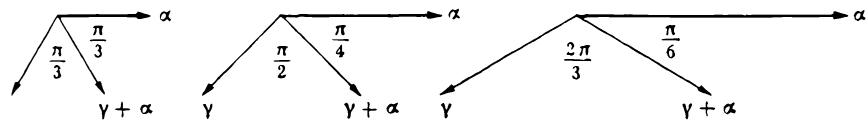
\includegraphics[keepaspectratio]{images/part001_d4d2d336.jpg}}

\begin{enumerate}
\def\labelenumi{\arabic{enumi})}
\setcounter{enumi}{2}
\tightlist
\item
  若 \(S\) 的长度为 2，则 \(n(\gamma, \alpha) = -2\)，因此
\end{enumerate}

\[
n (\alpha , \gamma) = - 1, (\alpha | \alpha) = \frac {1}{2} (\gamma | \gamma), (\alpha | \gamma) = - (\alpha | \alpha), \widehat {(\alpha , \gamma)} = \frac {3 \pi}{4}.
\]

\pandocbounded{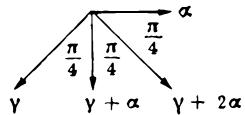
\includegraphics[keepaspectratio]{images/part001_f07fa75a.jpg}}

\begin{enumerate}
\def\labelenumi{\arabic{enumi})}
\setcounter{enumi}{3}
\tightlist
\item
  若 \(S\) 的长度为 3，则 \(n(\gamma, \alpha) = -3\)，因此
\end{enumerate}

\[
n (\alpha , \gamma) = - 1, (\alpha | \alpha) = \frac {1}{3} (\gamma | \gamma), (\alpha | \gamma) = - \frac {3}{2} (\alpha | \alpha), (\widehat {\alpha , \gamma}) = \frac {5 \pi}{6}.
\]

\pandocbounded{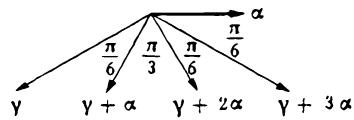
\includegraphics[keepaspectratio]{images/part001_9d247bec.jpg}}

我们将看到（Plate X, Systems \(A_{2}, B_{2}, G_{2}\)），所有这些情形实际上都能实现。

命题 10. 设 \(\alpha, \beta\) 是两个不成比例的根，且 \(\beta + \alpha\) 是一个根。设 \(p, q\) 是命题 9 中的整数。则

\[
\frac {(\beta + \alpha | \beta + \alpha)}{(\beta | \beta)} = \frac {q + 1}{p}.
\]

设 \(S\) 是 \(\alpha\)-链，由 \(\beta\) 定义，\(\gamma\) 是其起点；其长度 \(l\) 满足 \(\geqslant 1\)，因为 \(\beta + \alpha\) 是根。可能的情形如下：

\begin{enumerate}
\def\labelenumi{\arabic{enumi})}
\item
  \(l = 1\)；于是 \(\beta = \gamma, q = 0, p = 1, (\beta + \alpha | \beta + \alpha) = (\beta | \beta)\)。
\item
  \(l = 2\)，\(\beta = \gamma\)；于是 \(q = 0\)，\(p = 2\)，\((\beta + \alpha|\beta + \alpha) = \frac{1}{2} (\beta|\beta)\)。
\item
  \(l = 2, \beta = \gamma + \alpha\)；于是 \(q = 1, p = 1, (\beta + \alpha|\beta + \alpha) = 2(\beta|\beta)\)。
\item
  \(l = 3, \beta = \gamma\)；于是 \(q = 0, p = 3, (\beta + \alpha | \beta + \alpha) = \frac{1}{3} (\beta | \beta)\)。
\item
  \(l = 3, \beta = \gamma + \alpha\)；于是 \(q = 1, p = 2, (\beta + \alpha|\beta + \alpha) = (\beta|\beta)\)。
\item
  \(l = 3\)，\(\beta = \gamma + 2\alpha\)；于是 \(q = 2, p = 1\)，\((\beta + \alpha|\beta + \alpha) = 3(\beta|\beta)\)。
\end{enumerate}

每种情形都满足待证公式。

命题 11. 假设 R 不可约。设 \(\alpha\) 和 \(\beta\) 是满足 \(\| \alpha \| = \| \beta \|\) 的两个根。存在 \(g \in \mathrm{W}(\mathbb{R})\)，使得 \(g(\alpha) = \beta\)。

根 \(\alpha\) 在 W(R) 下的变换生成 V（no. 2, Cor. of Prop. 5）。因此存在 \(g \in \mathrm{W}(\mathbb{R})\)，使得 \((g(\alpha)|\beta) \neq 0\)。从现在起假设 \((\alpha|\beta) \neq 0\)。由第 1 号的公式 (9)，\(n(\alpha, \beta) = n(\beta, \alpha)\)。必要时将 \(\beta\) 换成 \(s_{\beta}(\beta) = -\beta\)，可假设 \(n(\alpha, \beta) > 0\)。于是，根据第 3 号开头的列表，要么 \(\alpha = \beta\)（此时命题显然成立），要么 \(n(\alpha, \beta) = n(\beta, \alpha) = 1\)；在后一情形中

\[
s _ {\alpha} s _ {\beta} s _ {\alpha} (\beta) = s _ {\alpha} s _ {\beta} (\beta - \alpha) = s _ {\alpha} (- \beta - \alpha + \beta) = \alpha .
\]

\subsection{约化根系}

称根系是约化的，如果系统的每个根都是不可分根（no. 3）。

命题 12. 假设 R 不可约且约化。

\begin{enumerate}
\def\labelenumi{(\roman{enumi})}
\item
  比值 \(\frac{(\beta|\beta)}{(\alpha|\alpha)}\) 对 \(\alpha \in \mathbb{R}, \beta \in \mathbb{R}\) 必须取 \(1, 2, \frac{1}{2}, 3, \frac{1}{3}\) 中的一个值。
\item
  集合 \((\alpha |\alpha)\)（其中 \(\alpha \in \mathrm{R}\)）至多含有两个元素。
\end{enumerate}

由于 R 不可约，根在 W(R) 下的变换生成 V（no. 2, Cor. of Prop. 5）。因此，对任意根 \(\alpha, \beta\)，存在一个根 \(\beta'\)，使得 \((\alpha|\beta') \neq 0\) 且 \((\beta'|\beta') = (\beta|\beta)\)。由第 1 号的公式 (9) 及第 3 号的列表，\(\frac{(\beta'|\beta')}{(\alpha|\alpha)}\) 取 \(1, 2, \frac{1}{2}, 3, \frac{1}{3}\) 中的一个值（回顾一下，系统假设为约化的）。将 \((x|y)\) 乘以适当的标量，可以假设对于某些根 \((\alpha|\alpha) = 1\)，而 \((\beta|\beta)\) 对 \(\beta \in \mathbb{R}\) 的其他可能值为 2 和 3。2 和 3 不可能同时取得，因为在这种情况下会存在 \(\beta \in \mathbb{R}, \gamma \in \mathbb{R}\)，使得 \(\frac{(\gamma|\gamma)}{(\beta|\beta)} = \frac{3}{2}\)，这与我们上面看到的相矛盾。

命题 13. 假设 R 不可约、非约化且秩 \(\geqslant 2\)。

\begin{enumerate}
\def\labelenumi{(\roman{enumi})}
\item
  不可分根的集合 \(\mathbf{R}_0\) 是 V 中的根系；该系统不可约且约化；并且 \(\mathrm{W}(\mathrm{R}_0) = \mathrm{W}(\mathrm{R})\)。
\item
  设 \(\mathbf{A}\) 是根 \(\alpha\) 的集合，其中 \((\alpha |\alpha)\) 取最小值 \(\lambda\)。则 \(\mathbf{A}\) 中任意两个不成比例的元素都正交。
\item
  设 B 是 \(\beta \in \mathbb{R}\) 的集合，满足 \((\beta |\beta) = 2\lambda\)。则 \(B \neq \emptyset\)，\(R_0 = A \cup B\)，\(R = A \cup B \cup 2A\)。
\end{enumerate}

若 \(\alpha \in \mathbb{R} - \mathbb{R}_0\)，则 \(\frac{1}{2}\alpha \in \mathbb{R}\)，但 \(\frac{1}{2}\left(\frac{1}{2}\alpha\right) \notin \mathbb{R}\)（命题 8），所以 \(\frac{1}{2}\alpha \in \mathbb{R}_0\)。这证明了 \(\mathbb{R}_0\) 满足 \((\mathrm{RS}_1)\)。显然，对所有 \(\alpha \in \mathbb{R}\)，\(s_{\alpha, \alpha'}(\mathbb{R}_0) = \mathbb{R}_0\)，所以 \(\mathbb{R}_0\) 满足 \((\mathrm{RS}_{II})\) 和 \((\mathrm{RS}_{III})\)。由于 \(\alpha \in \mathbb{R} - \mathbb{R}_0\) 蕴含 \(\frac{1}{2}\alpha \in \mathbb{R}_0\)，且 \(s_\alpha = s_{\alpha/2}\)，我们有 \(\mathrm{W}(\mathrm{R}) = \mathrm{W}(\mathrm{R}_0)\)。因此 \(\mathbb{R}_0\) 不可约（命题 5 的推论），且显然是约化的。

由于 R 不是约化的，存在 \(\alpha\in R_{0}\)，使得 \(2\alpha\in R\)。由于 \(R_{0}\) 不可约且 \(\dim V\geqslant2\)，\(\alpha\) 不可能与每个根成比例或正交。取 \(\beta\in R_{0}\)，使得 \(n(\beta,\alpha)\neq0\)，且 \(\beta\) 不与 \(\alpha\) 成比例。必要时将 \(\beta\) 换成 \(-\beta\)，可假设 \(n(\beta,\alpha)>0\)。现在 \(\frac{1}{2}n(\beta,\alpha)=n(\beta,2\alpha)\in\mathbf{Z}\)，所以 \(n(\beta,\alpha)\in2\mathbf{Z}\)。由第 3 号的列表，\(n(\beta,\alpha)=2\)，\((\beta|\beta)=2(\alpha|\alpha)\)。由于 \(R_{0}\) 约化，命题 12 表明，对所有 \(\gamma\in R_{0}\)，要么 \((\gamma|\gamma)=(\alpha|\alpha)\)，要么 \((\gamma|\gamma)=2(\alpha|\alpha)\)。此外，上面表明，对所有 \(\gamma\in R-R_{0}\)，向量 \(\frac{1}{2}\gamma\) 是 \(R_{0}\) 的元素，且 \(\left(\frac{1}{2}\gamma|\frac{1}{2}\gamma\right)=(\alpha|\alpha)\)。因此，\(\lambda=(\alpha|\alpha)\)，\(B\neq\varnothing\)，\(R_{0}=A\cup B\)，且 \(R\subseteq A\cup B\cup2A\)；另一方面，若 \(\gamma\in A\)，则存在 \(g\in W(R)\)，使得 \(\gamma=g(\alpha)\)（命题 11），所以 \(2\gamma=g(2\alpha)\in R\)；于是 \(2A\subseteq R\)，且 \(R=A\cup B\cup2A\)。最后，设 \(\gamma,\gamma'\) 是 A 中两个不成比例的元素。于是

\[
n (2 \gamma , \gamma^ {\prime}) = 2 n (\gamma , \gamma^ {\prime}) = 4 n (\gamma , 2 \gamma^ {\prime}) \in 4 \mathbf {Z}, \text { and } | n (\gamma , \gamma^ {\prime}) | \leqslant 1
\]

因为 \(\gamma\) 和 \(\gamma'\) 长度相同，所以 \(n(\gamma, \gamma') = 0\)，且 \((\gamma|\gamma') = 0\)。

命题 14. 假设 R 不可约且约化，并且 \((\alpha|\alpha)\) 取值为 \(\lambda\) 和 \(2\lambda\)，其中 \(\alpha\in R\)。设 A 是根 \(\alpha\) 的集合，满足 \((\alpha|\alpha)=\lambda\)。假设 A 中任意两个不成比例的元素都正交。则 \(R_{1}=R\cup2A\) 是不可约的非约化根系，而 R 是 \(R_{1}\) 的不可分根的集合。

显然，\(R_{1}\) 满足 \((RS_{I})\) 和 \((RS_{III})\)。我们证明，若 \(\alpha, \beta \in R_{1}\)，则 \(\langle\alpha^{\sim}, \beta\rangle \in Z\)。当 \(\alpha \in R\) 时这显然成立。由于 \((2\alpha)^{\sim} = \frac{1}{2}\alpha^{\sim}\)（\(\alpha \in A\)），当 \(\alpha, \beta \in 2A\) 时也立即可得。最后，设 \(\beta \in R\)，且 \(\alpha = 2\gamma\)，其中 \(\gamma \in A\)。

\begin{enumerate}
\def\labelenumi{\arabic{enumi})}
\item
  若 \(\gamma = \pm \beta\)，则 \(\langle \alpha^{\prime},\beta \rangle = \pm \frac{1}{2}\langle \gamma^{\prime},\gamma \rangle = \pm 1\)。
\item
  若 \(\gamma\) 不与 \(\beta\) 成比例且 \(\beta \in A\)，根据 \(A\) 的假设，有 \(\langle \gamma^{\sim},\beta \rangle = 0\)，所以 \(\langle \alpha^{\sim},\beta \rangle = 0\)。
\item
  若 \(\beta \in \mathbb{R} - \mathbb{A}\)，则 \((\beta |\beta) = 2\lambda = 2(\gamma |\gamma)\)，所以根据第 3 号的列表，\(\langle \beta, \gamma^{\prime} \rangle\) 等于 0、2 或 -2。因此 \(\langle \beta, \alpha^{\prime} \rangle = \frac{1}{2}\langle \beta, \gamma^{\prime} \rangle \in \mathbf{Z}\)。
\end{enumerate}

因此 \(R_{1}\) 是 V 中的根系，其余断言显然。

\subsection{根系的室与基}

对所有 \(\alpha \in \mathbb{R}\)，令 \(L_{\alpha}\) 为 \(V\) 中由在 \(s_{\alpha}\) 下不变的点组成的超平面。由 \(V\) 中的这些 \(L_{\alpha}\) 所决定的室（Chap. V, § 1, no. 3）称为 \(R\) 的室。由 \(V \to V^{*}\) 这一由内积 \((x|y)\) 定义的双射将 \(\alpha\) 映为 \(\frac{2\alpha^{-}}{(\alpha^{-}|\alpha^{-})}\) 对 \(\alpha \in R\) 成立，因而将 \(L_{\alpha}\) 映为 \(L_{\alpha^{-}}\)，并因而将 \(R\) 的室映为 \(R^{-}\) 的室。若 \(C\) 是 \(R\) 的室，对应的 \(\mathbb{R}^{\sim}\) 的室记为 \(\mathbb{C}^{\sim}\)。由第 2 号的 Prop. 7，\(\mathbb{C}^{\sim}\) 只取决于 \(\mathbb{C}\)，而不取决于 \((x|y)\) 的选择。

定理 2. (i) 群 W(R) 在室的集合上单纯传递地作用。

\begin{enumerate}
\def\labelenumi{(\roman{enumi})}
\setcounter{enumi}{1}
\item
  设 \(\mathrm{C}\) 是一个室。于是 \(\overline{\mathrm{C}}\) 是 \(\mathrm{W}(\mathrm{R})\) 的基本域。
\item
  C 是一个开单纯形锥（Chap. V, § 1, no. 6）。
\item
  设 \(L_{1}, L_{2}, \ldots, L_{l}\) 是 C 的壁。对所有 i，存在唯一的不可分根 \(\alpha_{i}\)，使得 \(L_{i} = L_{\alpha_{i}}\)，并且 \(\alpha_{i}\) 与 C 位于 \(L_{i}\) 的同一侧。
\item
  集合 B(C) = \(\{\alpha_{1},\ldots,\alpha_{l}\}\) 是 V 的一个基。
\item
  C 是由 \(x \in V\) 构成的集合，满足 \(\langle \alpha_i, x \rangle > 0\) 对所有 \(i\) 成立（或等价地，是由 \(x \in V\) 构成的集合，满足 \((x|\alpha_i) > 0\) 对所有 \(i\) 成立）。
\item
  令 \(S\) 为 \(s_{\alpha_i}\) 的集合。则 \((W(R), S)\) 是一个 Coxeter 系统（Chap. IV, § 1, no. 3）。
\end{enumerate}

断言 (i) 和 (vii) 由 Chap. V, § 3, no. 2 的 Th. 1 得到。断言 (ii) 由 Chap. V, § 3, no. 3 的 Th. 2 得到。断言 (iv) 显然。根 \(\alpha_{i}\) 与 \(L_{i}\) 正交，而 \(\alpha_{i}^{-}\) 等同于 \(2\alpha_{i}/(\alpha_{i}|\alpha_{i})\)。由于 W(R) 是本质的（no. 1, Remark 3），断言 (iii)、(v) 和 (vi) 由 Chap. V, § 3, no. 9 的 Prop. 7 得到。

注记。1）断言 (vii) 特别表明，\(\mathrm{W}(\mathbb{R})\) 由反射 \(s_{\alpha_i}\) 生成。

\begin{enumerate}
\def\labelenumi{\arabic{enumi})}
\setcounter{enumi}{1}
\item
  若 \(x, y \in \mathbb{C}\)，则 \((x|y) > 0\)（Chap. V, § 3, no. 5, Lemma 6），换言之，角 \((\widehat{x,y})\) 是锐角。
\item
  令 \(m(\alpha, \beta)\) 为 \(s_{\alpha} s_{\beta} (\alpha, \beta \in \mathrm{B}(\mathrm{C}))\) 的阶。矩阵 \((m(\alpha, \beta))\) 与 (W, S) 的 Coxeter 矩阵（Chap. IV, § 1, no. 9）等同。若 \(\alpha \neq \beta\)，Chap. V, § 3, no. 4 的 Prop. 3 表明，角 \((\widehat{\alpha, \beta})\) 等于 \(\pi - \frac{\pi}{m(\alpha, \beta)}\)；特别地，这个角要么是钝角，要么等于 \(\pi\)，并且 \((\alpha | \beta) \leqslant 0\)。利用第 3 号的列表，得到 \(m(\alpha, \beta)\) 等于 2、3、4 或 6。
\end{enumerate}

定义 2. R 的子集 B 称为 R 的一个基，如果存在 R 的一个室 C，使得 B = B(C)。若 C 是一个室，则 B(C) 称为由 C 定义的 R 的基。

注记。4）Th. 2 的断言 (vi) 表明，映射 C ↦ B(C) 是从室的集合到基的集合的双射。因此，W(R) 在基的集合上单纯传递地作用。

\begin{enumerate}
\def\labelenumi{\arabic{enumi})}
\setcounter{enumi}{4}
\tightlist
\item
  设 C 是 R 的一个室，B 是相应的基。若 \(\alpha\in B\)，置 \(\varphi(\alpha)=\alpha^{-}\)（当 \(2\alpha\notin R\) 时），置 \(\varphi(\alpha)=\frac{1}{2}\alpha^{-}\)（当 \(2\alpha\in R\) 时）。于是 \(\varphi(B)\) 是 \(R^{-}\) 的基，由 \(C^{-}\) 定义；这是因为 \(C^{-}\) 的壁是 \(L_{\alpha^{-}}\)，对 \(\alpha\in B\) 成立。
\end{enumerate}

定义 3. 设 B 是 R 的一个基。R 的 Cartan 矩阵（相对于 B）是矩阵 \((n(\alpha,\beta))_{\alpha,\beta\in\mathbb{B}}\)。

对所有 \(\alpha \in \mathrm{B}\)，\(n(\alpha, \alpha) = 2\)。对于 \(\alpha, \beta \in \mathrm{B}\)，

\[
n (\alpha , \beta) = 2 \frac {(\alpha | \beta)}{(\beta | \beta)} = - 2 \frac {\| \alpha \|}{\| \beta \|} \cos \frac {\pi}{m (\alpha , \beta)},\tag{11}
\]

其中 \(m(\alpha, \beta)\) 如上所述表示 \(s_{\alpha}s_{\beta}\) 的阶。若 \(\alpha \neq \beta\)，则 \(n(\alpha, \beta) = 0\)、-1、-2 或 -3（cf.~no. 3）。

注记。6）Cartan 矩阵 \((n(\alpha,\beta))\) 不应与 Coxeter 矩阵 \((m(\alpha,\beta))\) 混淆。特别要注意，Cartan 矩阵不一定是对称的。

\begin{enumerate}
\def\labelenumi{\arabic{enumi})}
\setcounter{enumi}{6}
\tightlist
\item
  典范编号。若 B 和 \(\mathbf{B}'\) 是 R 的两个基，则存在唯一的 \(w \in \mathbf{W}\)，使得 \(w(\mathbf{B}) = \mathbf{B}'\)。有
\end{enumerate}

\[
n (w (\alpha), w (\beta)) = n (\alpha , \beta) \text { and } m (w (\alpha), w (\beta)) = m (\alpha , \beta)
\]

对于 \(\alpha, \beta \in \mathbf{B}\)。因此，与 B 相关的 Cartan 矩阵和 Coxeter 矩阵可以通过与 \(\mathbf{B}'\) 相关的矩阵同双射的复合得到。

\[
\alpha \mapsto w (\alpha)
\]

从 B 到 B' 得到。

Cartan 矩阵和 Coxeter 矩阵实际上可以按下述方式典范地定义。令 X 是二元组 \((B, \alpha)\) 的集合，其中 B 是 R 的一个基且 \(\alpha \in B\)。群 W 以显然的方式作用于 X，并且 W 在 X 上的每个轨道与集合 \(\{B\} \times B\) 中的每一个恰好交于一点。若 I 是这些轨道的集合，则每个基 B 都有一个典范编号 \((\alpha_{i})_{i \in I}\)。此外，存在唯一的矩阵 \(N = (n_{ij})\)（相应地，\(M = (m_{ij})\)），其类型为 \(I \times I\)，使得对于任意基 B，与 B 相关的 Cartan 矩阵（相应地，Coxeter 矩阵）都可以通过与 B 的典范编号复合而由 N（相应地，M）得到；这个矩阵称为 R 的典范 Cartan 矩阵（相应地，典范 Coxeter 矩阵）。

命题 15. 设 B 是 R 的一个基，\(\alpha\) 是一个不可分根。存在 \(\beta \in B\) 和 \(w \in W(R)\)，使得 \(\alpha = w(\beta)\)。

设 C 是满足 \(\mathrm{B} = \mathrm{B}(\mathrm{C})\) 的室。超平面 \(L_{\alpha}\) 是 R 的某个室 \(C'\) 的一个壁，并且存在 \(\mathrm{W}(\mathrm{R})\) 中的元素将 \(C'\) 变换为 C。因此可以归结到 \(L_{\alpha}\) 是 C 的一个壁的情形。于是 \(\alpha\) 与 R 中的某个元素 \(\beta\) 成比例。由于 \(\alpha\) 和 \(\beta\) 都不可分，\(\alpha = \pm\beta\)。若 \(\alpha = -\beta\)，则 \(\alpha = s_{\beta}(\beta)\)，故命题得证。

推论。设 \(R_{1}\) 和 \(R_{2}\) 是分别位于向量空间 \(V_{1}\) 和 \(V_{2}\) 中的两个约化根系，设 \(B_{1}\) 和 \(B_{2}\) 是 \(R_{1}\) 和 \(R_{2}\) 的基。设 \(f: B_{1} \to B_{2}\) 是一个将 \(R_{1}\) 的 Cartan 矩阵变为 \(R_{2}\) 的 Cartan 矩阵的双射。则存在

存在一个同构 \(\mathrm{F}: \mathrm{V}_1 \to \mathrm{V}_2\)，将 \(\mathbb{R}_1\) 变为 \(\mathbb{R}_2\)，并将 \(\alpha\) 变为 \(f(\alpha)\)，对所有 \(\alpha \in \mathbb{B}_1\) 成立。

设 F 是从 \(V_{1}\) 到 \(V_{2}\) 的同构，将 \(\alpha\) 变为 \(f(\alpha)\)，对所有 \(\alpha \in B_{1}\) 成立。于是 F 将 \(s_{\alpha}\) 变为 \(s_{f(\alpha)}\)，从而将 \(W(R_{1})\) 变为 \(W(R_{2})\)（Th. 2），进而将 \(R_{1}\) 变为 \(R_{2}\)（命题 15）。

命题 16. 设 B 是 R 的一个基，G 是 A(R) 中由保持 B 不变的元素组成的子群。则 W(R) 是 A(R) 的正规子群，而 A(R) 是 G 与 W(R) 的半直积。

若 \(\alpha\in R\) 且 \(t\in\mathrm{A}(\mathrm{R})\)，则 \(ts_{\alpha}t^{-1}=s_{t(\alpha)}\)；由于 \(\mathrm{W}(\mathrm{R})\) 由 \(s_{\alpha}\) 生成，我们看到 \(\mathrm{W}(\mathrm{R})\) 是 \(\mathrm{A}(\mathrm{R})\) 的正规子群。由结构输运，\(\mathrm{A}(\mathrm{R})\) 将 R 的一个基变换为 R 的一个基。由于 \(\mathrm{W}(\mathrm{R})\) 在基的集合上单纯传递地作用，\(\mathrm{A}(\mathrm{R})\) 的每个元素都可以唯一地写成 \(g_{1}g_{2}\) 的形式，其中 \(g_{1}\in\mathrm{W}(\mathrm{R})\)，\(g_{2}\in G\)。

注记。8）设 \(\mathbb{R}_1, \ldots, \mathbb{R}_p\) 是分别位于向量空间 \(\mathbb{V}_1, \ldots, \mathbb{V}_p\) 中的根系，\(\mathbb{R}\) 是 \(\mathbb{R}_i\) 在 \(\mathbb{V} = \prod_i \mathbb{V}_i\) 中的直和，\(\mathbb{C}_i\) 是 \(\mathbb{R}_i\) 的一个室，且 \(\mathbb{B}_i = \mathbb{B}(\mathbb{C}_i)\)。显然 \(\mathbb{C} = \prod_i \mathbb{C}_i\) 是 \(\mathbb{R}\) 的一个室，且 \(\mathbb{B}(\mathbb{C}) = \bigcup_i \mathbb{B}_i\)。由 Th. 2，\(\mathbb{R}\) 的所有室和基都以这种方式得到。

\subsection{正根}

设 C 是 R 的一个室，且 \(\mathrm{B}(\mathrm{C})=\{\alpha_{1},\ldots,\alpha_{l}\}\) 是相应的 R 的基。由 C 在 V（相应地，在 \(V^{*}\)）上定义的序关系，是与 V（相应地，与 \(V^{*}\)）的向量空间结构相容的序关系，并且其中满足 \(\geqslant0\) 的元素是 \(\alpha_{i}\)（相应地，\(\alpha_{i}^{-}\)）的线性组合，且系数为 \(\geqslant0\)。在这些序关系之一中为正的元素称为关于 C 正，或关于基 \(\mathrm{B}(\mathrm{C})\) 正。这些序关系也由 \(C^{-}\) 定义，正如将 V 与 \(V^{*}\) 等同并使用在 \(\mathrm{W}(\mathrm{R})\) 下不变的内积所看到的。根据 Th. 2, no. 5，\(V^{*}\) 中的元素是 \(\geqslant0\) 当且仅当其在 C 上的取值为 \(\geqslant0\)。V 中的元素 x 是 \(\geqslant0\) 当且仅当它在 \(C^{-}\) 上的取值为 \(\geqslant0\)，或者等价地，当且仅当 \((x|y)\geqslant0\) 对所有 \(y\in C\) 成立。

\(\overline{C}\) 的元素是 \(\geqslant 0\)（相对于 \(C\)），由 Chap. V, § 3, no. 5 的 Lemma 6 可知。但是，\(\geqslant 0\) 的元素集合（相对于 \(C\)）一般不同于 \(\overline{C}\)（cf.~Plate X, Systems \(A_2\) 、\(B_2\) 、\(G_2\)）。

定理 3. 每个根都是 B(C) 中元素的同号整数系数组合。特别地，每个根关于 C 不是正的就是负的。

若 \(\alpha \in \mathbb{R}\)，则 \(L_{\alpha}\) 是 \(\alpha\) 的核，不与 \(C^{\cdot}\) 相交，因此 \(\alpha\) 要么为 \(>0\)（在整个 \(C^{\cdot}\) 上），要么为 \(< 0\)（在整个 \(C^{\cdot}\) 上），从而得到第二个断言。还需证明 \(\alpha\) 属于子群 \(P\)，它是 \(V\) 中由 \(B(C)\) 生成的子群；可以假设 \(\alpha\) 不可分。现在群 P 显然在 \(s_{\gamma}\) 下保持不变，其中 \(\gamma \in \mathrm{B}(\mathrm{C})\)，因而根据 Th. 2 也在 \(\mathrm{W}(\mathrm{R})\) 下保持不变。由于 \(\alpha\) 具有 \(w(\beta)\) 的形式，其中 \(w \in \mathrm{W}(\mathrm{R})\) 且 \(\beta \in \mathrm{B}(\mathrm{C})\)（cf.~命题 15），所以 \(\alpha \in P\)。证毕。

记 \(R_{+}(C)\) 为关于 C 为正的根的集合。于是，

\[
R = R _ {+} (C) \cup (- R _ {+} (C))
\]

是 \(R\) 的一个划分。

推论。设 \(\gamma\) 是根的整数系数组合，\(\alpha\) 是不可分根。若 \(\gamma\) 与 \(\alpha\) 成比例，则 \(\gamma \in Z\alpha\)。

由第 5 号的命题 15，可以选择 C 使得 \(\alpha \in B(C)\)。由定理 3，

\[
\gamma = \sum_ {\beta \in B (C)} n _ {\beta} \beta \text {with} n _ {\beta} \in \mathbf {Z}.
\]

因此，若 \(\gamma\) 与 \(\alpha\) 成比例，则 \(\gamma = n_{\alpha}\alpha\)，这就证明了该推论。

现在令 S 为反射 \(s_{\alpha}\) 的集合，其中 \(\alpha \in \mathrm{B}(\mathrm{C})\)，并令 T 为 S 在 W 下的共轭元素的并集。对于 \(\alpha \in \mathrm{B}(\mathrm{C})\) 和 \(w \in W\)，T 中的元素 \(t = ws_{\alpha}w^{-1}\) 是正交反射 \(s_{\beta}\)，其中根 \(\beta = w(\alpha)\)；反过来，对于任意不可分根 \(\beta\)，存在 \(w \in W\)，使得 \(\alpha = w^{-1}(\beta) \in \mathrm{B}(\mathrm{C})\)（命题 15），并且 \(s_{\beta} = ws_{\alpha}w^{-1} \in T\)。因此，得到一个双射 \(\psi\)，从不可分根集合到 \(\{\pm1\} \times T\)，它把不可分根 \(\beta\) 对应到二元组 \((\varepsilon, s_{\beta})\)，其中 \(\varepsilon = +1\) 当 \(\beta\) 为正，且 \(\varepsilon = -1\) 当 \(\beta\) 为负。

另一方面，(W, S) 是一个 Coxeter 系统（定理 2），可以应用 Chap. IV, § 1, no. 4 的结果。我们已经看到，若 w 是 W 中长度（相对于 S）为 q 的元素，则存在一个含有 q 个元素的 T 的子集 \(T_{w}\)，使得当 \(w = s_{1} \ldots s_{q}\)，其中 \(s_{i} \in S\)，并且

\[
t _ {i} = s _ {1} \dots s _ {i - 1} s _ {i} s _ {i - 1} \dots s _ {1}
\]

（对于 \(1 \leqslant i \leqslant q\)），则 \(\mathrm{T}_w = \{t_1, \ldots, t_q\}\)。回顾一下，我们还在第 1 节第 4 号定义了一个数 \(\eta(w, t)\)，当 \(w \in \mathrm{W}\) 且 \(t \in \mathrm{T}\) 时，其值为 \(+1\)（当 \(t \notin \mathrm{T}_w\) 时），为 \(-1\)（当 \(t \in \mathrm{T}_w\) 时）。最后，回顾一下，如果我们用下式定义映射 \(\mathrm{U}_w\)，从集合 \(\{\pm 1\} \times \mathrm{T}\) 到自身，

\[
\mathbf {U} _ {w} (\varepsilon , t) = (\varepsilon \eta (w ^ {- 1}, t), w t w ^ {- 1}),
\]

映射 \(w \mapsto \mathrm{U}_w\) 是从 \(W\) 到集合 \(\{\pm 1\} \times T\) 的置换群的同态（Chap. IV, §1, no. 4, Lemma 1）。

命题 17. 假设 R 是约化的，并令 \(w \in W\)、\(\alpha \in R\)。

\begin{enumerate}
\def\labelenumi{(\roman{enumi})}
\item
有 \(\psi(w(\alpha)) = U_w(\psi(\alpha)).\)
\item
  假设 \(\alpha\) 为正。根 \(w(\alpha)\) 为负，当且仅当
\end{enumerate}

\[
\eta (w ^ {- 1}, s _ {\alpha}) = - 1,
\]

换言之，当 \(s_{\alpha} \in \mathrm{T}_{w^{-1}}\) 时。

\begin{enumerate}
\def\labelenumi{(\roman{enumi})}
\setcounter{enumi}{2}
\tightlist
\item
当且仅当 \(\eta(w,s_{\alpha})=-1\)，室 C 和 \(w(C)\) 位于超平面 \(L_{\alpha}\) 的两侧。换言之，集合 \(T_{w}\) 由分隔 C 和 \(w(C)\) 的各壁对应的反射组成。
\end{enumerate}

设 \(\beta \in \mathrm{B}(\mathrm{C})\)，并置 \(s = s_{\beta}\)。显然 \(\mathrm{T}_s = \{s\}\)，从而

\[
\mathrm{U} _ {s} (\varepsilon , t) = \left\{ \begin{array}{l l} (\varepsilon , s t s ^ {- 1}) & \text { if } t \neq s \\ (- \varepsilon , s) & \text { if } t = s. \end{array} \right.\tag{12}
\]

另一方面，设 \(\rho = \sum_{\gamma \in B(C)} n_{\gamma}(\rho) \gamma\) 是一个正根。置

\[
s (\rho) = \sum_ {\gamma \in B (C)} n _ {\gamma} (s (\rho)) \gamma .
\]

若 \(\rho \neq \beta\)，则存在 \(\gamma \in \mathrm{B}(\mathbf{C})\)，满足 \(\gamma \neq \beta\)，使得 \(n_{\gamma}(\rho) > 0\)，并且有 \(n_{\gamma}(s(\rho)) = n_{\gamma}(\rho) > 0\)（第 1 号的公式 (5)）。因此 \(s(\rho)\) 是正的。立即得到

\[
\psi (s (\varepsilon . \rho)) = \left\{ \begin{array}{l l} (\varepsilon , s s _ {\rho} s ^ {- 1}) & \text {if} \rho \neq \beta \\ (- \varepsilon , s) & \text {if} \rho = \beta . \end{array} \right.\tag{13}
\]

比较 (12) 和 (13) 现在表明 \(\mathrm{U}_{s}(\psi(\gamma)) = \psi(s(\gamma))\) 对所有根 \(\gamma\) 及所有 \(s \in S\) 成立。由于 S 生成 W，(i) 得证。

另一方面，称 \(w(\alpha)\) 为负，等价于

\[
\psi (w (\alpha)) = (- 1, w s _ {\alpha} w ^ {- 1}),
\]

或者根据 (i)，等价于 \(\mathrm{U}_w(\psi (\alpha)) = (-1, ws_{\alpha}w^{-1})\)。如果此外 \(\alpha\) 为正，则 \(\psi (\alpha) = (+1,s_{\alpha})\)，且 \(\mathrm{U}_w(\psi (\alpha)) = (\eta (w^{-1},s_{\alpha}),ws_{\alpha}w^{-1})\)，故得到 (ii)。

最后，根据 (ii)，\(\eta(w,s_{\alpha})=-1\) 当且仅当根 \(\alpha\) 和 \(w^{-1}(\alpha)\) 中一个为正而另一个为负。这等价于 \((\alpha|x).(w^{-1}(\alpha)|x)=(\alpha|x).( \alpha|w(x))<0\) 对所有 \(x\in C\) 成立，从而得到 (iii) 的第一个断言。(iii) 的第二个断言立即可得。

推论 1. 设 \(\beta \in \mathrm{B}(\mathbb{C})\)。反射 \(s_{\beta}\) 将与 \(\beta\) 不成比例的正根进行置换。

我们立即归结到 R 约化的情形。在这种情况下，我们的断言由 (ii) 以及 \(T_{s_{\beta}} = s_{\beta}\) 这一事实得到。

推论 2. 假设 R 是约化的。设 \(w \in W\)，设 \(q\) 是 \(w\) 关于 S 的长度（Chap. IV, § 1, no. 1），并设 \(w = s_1 \ldots s_q\) 是 \(w\) 的一个约化分解。设 \(\alpha_1, \ldots, \alpha_q\) 是 B(C) 中与 \(s_1, \ldots, s_q\) 对应的元素。置

\[
\theta_ {i} = s _ {q} s _ {q - 1} \dots s _ {i + 1} (\alpha_ {i}), \quad i = 1, \dots , q.
\]

根 \(\theta_{i}\) 都 \(>0\)、彼此不同，\(w(\theta_{i}) < 0\)，并且每个满足 \(\alpha > 0\) 且 \(w(\alpha) < 0\) 的根都等于某个 \(\theta_{i}\)。

令 \(X\) 为满足 \(\alpha > 0\) 且 \(w(\alpha) < 0\) 的根的集合。由 (ii)，

\[
\operatorname{Card} (X) = \operatorname{Card} \left(T _ {w ^ {- 1}}\right) = l \left(w ^ {- 1}\right) = l (w) = q.
\]

另一方面，若 \(\alpha \in X\)，显然存在 \(i \in [1, q]\)，使得

\[
s _ {i + 1} \ldots s _ {q} (\alpha) > 0 \quad \text {and} \quad s _ {i} s _ {i + 1} \ldots s _ {q} (\alpha) <   0.
\]

由 Cor. 1，这意味着 \(s_i s_{i+1} \ldots s_q(\alpha) = \alpha_i\)，因而 \(\alpha = \theta_i\)。于是集合 X 包含于 \(\theta_i\) 的集合中。由于 \(\text{Card}(X) = q\)，这只有在 X 等于 \(\theta_i\) 的集合且这些元素彼此不同时才可能。因此推论得证。

推论 3. 假设 R 是约化的。W 中存在唯一的最长元素 \(w_0\)。它的长度等于正根的数目，并且 \(w_0\) 将室 C 变为 -C。我们有 \(w_0^2 = 1\)，且 \(l(ww_0) = l(w_0) - l(w)\) 对所有 \(w \in W\) 成立。

显然 -C 是一个室。因此存在 W 中的元素 \(w_{0}\) 将 C 变为 -C。于是 \(w_{0}(\alpha) < 0\) 对所有正根 \(\alpha\) 成立，推论 3 的前两个断言立即由推论 2 得到。我们有 \(w_{0}^{2}(C) = C\)，所以 \(w_{0}^{2} = 1\)。最后，若 \(w \in W\)，则由命题 17 (iii)，长度 \(l(w)\)（相应地，\(l(ww_{0})\)）等于分隔 C 与 \(w(C)\)（相应地，\(ww_{0}(C) = -w(C)\)）的壁数。由于 \(w(C)\) 和 \(-w(C)\) 位于每一面墙的两侧，\(l(w) + l(w_{0})\) 等于墙的总数，也就是 \(l(w_{0})\)。

命题 18. 设 \(x \in V\)。以下三个性质等价：

\begin{enumerate}
\def\labelenumi{(\roman{enumi})}
\item
  \(x \in \overline{C};\)
\item
  \(x \geqslant s_{\alpha}(x)\) 对所有 \(\alpha \in \mathrm{B}(\mathrm{C})\) 成立（相对于 \(\mathrm{C}\) 定义的序关系）；
\item
   \(x \geqslant w(x)\) 对所有 \(w \in W\) 成立。
\end{enumerate}

由于 \(s_{\alpha}(x) = x - \langle x, \alpha' \rangle \alpha\)，且 \(\overline{\mathbf{C}}\) 是由 \(x \in V\) 构成的集合，满足 \(\langle x, \alpha' \rangle \geqslant 0\) 对所有 \(\alpha \in \mathrm{B}(\mathbf{C})\) 成立，(i) 与 (ii) 的等价性显然。另一方面，显然 (iii) \(\Longrightarrow\) (ii)。我们证明 (i) \(\Longrightarrow\) (iii)。设 \(x \in \overline{\mathbf{C}}\)，且 \(w \in W\)。我们对长度 \(l(w)\) 的 \(w\) 归纳。\(l(w) = 0\) 的情形是平凡的。若 \(l(w) \geqslant 1\)，则 \(w\) 可写成 \(w = w's_{\alpha}\) 的形式，其中 \(\alpha \in \mathrm{B}(\mathbf{C})\) 且 \(l(w') = l(w) - 1\)。于是

\[
x - w (x) = x - w ^ {\prime} (x) + w ^ {\prime} \left(x - s _ {\alpha} (x)\right).
\]

归纳假设表明 \(x - w'(x)\) 是正的。另一方面，

\[
w ^ {\prime} (x - s _ {\alpha} (x)) = w \left(s _ {\alpha} (x) - x\right) = - \langle x, \alpha^ {*} \rangle w (\alpha).
\]

现在 \(s_{\alpha} \in T_{w^{-1}}\)，命题 17 (ii) 表明 \(w(\alpha) < 0\)。故结论成立。

推论。元素 \(x \in \mathbf{C}\) 当且仅当有 \(x > w(x)\) 对所有 \(w \in \mathbf{W}\) 且 \(w \neq 1\) 成立。

命题 19. 设 \((\beta_{i})_{1\leqslant i\leqslant n}\) 是关于室 C 的正根序列，且 \(\beta_{1}+\beta_{2}+\cdots+\beta_{n}\) 是一个根。则存在置换 \(\pi\in S_{n}\)，使得对所有 \(i\in\{1,2,\ldots,n\}\)，\(\beta_{\pi(1)}+\beta_{\pi(2)}+\cdots+\beta_{\pi(i)}\) 都是根。

我们对 n 归纳，\(n \leqslant 2\) 时命题显然。置 \(\beta = \beta_{1} + \cdots + \beta_{n}\)。于是 \(\sum_{i=1}^{n} (\beta | \beta_{i}) = (\beta | \beta) > 0\)，所以存在一个指标 k，使得 \((\beta | \beta_{k}) > 0\)。若 \(\beta = \beta_{k}\)，则 n = 1，因为对所有 i 都有 \(\beta_{i} > 0\)。否则 \(\beta - \beta_{k}\) 是一个根（第 3 号的 Th. 1 的 Cor.）；于是只需将归纳假设应用于 \(\beta - \beta_{k} = \sum_{i \neq k} \beta_{i}\)。

推论 1. 设 \(\alpha \in \mathrm{R}_{+}(\mathrm{C})\)。则 \(\alpha \in \mathrm{B}(\mathrm{C})\)，当且仅当 \(\alpha\) 是两个正根之和。

若 \(\alpha\) 是两个正根之和，则定理 3 表明 \(\alpha \in \mathrm{B}(\mathrm{C})\)。若 \(\alpha \notin \mathrm{B}(\mathrm{C})\)，则定理 3 表明 \(\alpha = \sum_{k=1}^{n} \beta_k\)，其中 \(\beta_k \in \mathrm{B}(\mathrm{C})\) 对所有 \(k\) 成立，且 \(n \geqslant 2\)。必要时置换 \(\beta_k\)，可假设 \(\sum_{k=1}^{n-1}\) 是一个根（命题 19），因而 \(\alpha\) 是正根 \(\sum_{k=1}^{n-1} \beta_k\) 与 \(\beta_n\) 之和。

推论 2. 设 \(\varphi\) 是从 \(R\) 到交换群 \(\Gamma\) 的映射，具有以下性质：

\begin{enumerate}
\def\labelenumi{\arabic{enumi})}
\item
  \(\varphi(-\alpha) = -\varphi(\alpha)\) 对 \(\alpha \in \mathbf{R}\) 成立；
\item
  若 \(\alpha \in \mathrm{R}\)、\(\beta \in \mathrm{R}\) 且 \(\alpha + \beta \in \mathrm{R}\)，则 \(\varphi(\alpha + \beta) = \varphi(\alpha) + \varphi(\beta)\)。
\end{enumerate}

令 \(\mathbf{Q}\) 为 \(\mathbf{V}\) 中由 \(\mathbf{R}\) 生成的子群。于是 \(\varphi\) 延拓为从 \(\mathbf{Q}\) 到 \(\Gamma\) 的同态。

设 B 是 R 的一个基。设 \(\psi\) 是从 Q 到 \(\Gamma\) 的唯一同态，并且在 B 上与 \(\varphi\) 一致。只需证明 \(\psi(\alpha) = \varphi(\alpha)\)，其中 \(\alpha\) 是相对于 B 的正根。我们有 \(\alpha = \beta_{1} + \cdots + \beta_{m}\)，其中对所有 i 都有 \(\beta_{i} \in B\)，且对所有 h 都有 \(\beta_{1} + \cdots + \beta_{h} \in R\)（命题 19）。我们对 m 归纳证明 \(\psi(\alpha) = \varphi(\alpha)\)。当 m = 1 时显然成立。归纳假设给出

\[
\psi \left(\beta_ {1} + \dots + \beta_ {m - 1}\right) = \varphi \left(\beta_ {1} + \dots + \beta_ {m - 1}\right),
\]

且我们有 \(\psi (\beta_m) = \varphi (\beta_m)\)，所以 \(\psi (\alpha) = \varphi (\alpha)\)，这就证明了该推论。

 对于满足 \(\alpha = \sum_{\beta \in \mathrm{B}(\mathbb{C})} n_{\beta} \beta\) 且属于 \(\mathbb{R}\) 的任意根，记 \(\Upsilon(\alpha)\) 为满足 \(\beta \in \mathrm{B}(\mathbb{C})\) 且 \(n_{\beta} \neq 0\) 的元素的集合。此外，注意到 \(\mathrm{B}(\mathbb{C})\) 可以与由 \(\mathrm{W}(\mathbb{R})\) 和 \(s_{\alpha_i}\) 构成的 Coxeter 系统的图的顶点集等同（cf.~Chap. IV, § 1, no. 9 and Chap. V, § 3, no. 2）。

推论 3. a) 设 \(\alpha \in \mathbb{R}\)。则 \(\mathrm{Y}(\alpha)\) 是 \(\mathrm{B}(\mathrm{C})\) 的连通子集（Chap. IV, Appendix）。

\begin{enumerate}
\def\labelenumi{\alph{enumi})}
\setcounter{enumi}{1}
\tightlist
\item
  设 Y 是 B(C) 的非空连通子集。则 \(\sum_{\beta\in Y}\beta\) 属于 R。
\end{enumerate}

为了证明 \(a\) )，可假设 \(\alpha\) 为正。我们对 \(\operatorname{Card}(\mathbf{Y}(\alpha))\) 归纳；当 \(\operatorname{Card}(\mathbf{Y}(\alpha)) = 1\) 时断言显然。由命题 19，存在 \(\beta \in \mathrm{B}(\mathrm{C})\)，使得 \(\alpha - \beta \in \mathrm{R}\)。令 \(p\) 为最大的满足 \(\geqslant 0\) 且 \(\gamma = \alpha - p\beta \in \mathrm{R}\) 的整数。由于 \(\gamma - \beta \notin \mathrm{R}\) 且 \(\gamma + p\beta \in \mathrm{R}\)，有 \((\gamma|\beta) \neq 0\)（命题 9）；因此 \(\beta\) 至少与 \(\mathbf{Y}(\gamma)\) 中的一个元素相连。但 \(\mathbf{Y}(\alpha) = \mathbf{Y}(\gamma) \cup \{\beta\}\)，且 \(\mathbf{Y}(\gamma)\) 根据归纳假设是连通的。因此 \(\mathbf{Y}(\alpha)\) 是连通的，这就证明了 \(a\) )。

现在设 Y 是 B(C) 的非空连通子集；我们对 \(\operatorname{Card}(Y)\) 归纳证明 \(\sum_{\beta\in Y}\beta\) 是一个根。\(\operatorname{Card}(Y)\leqslant1\) 的情形是平凡的。假设 \(\operatorname{Card}(Y)\geqslant2\)。由于 X 是一片森林（Chap. V, § 4, no. 8, Prop. 8），Y 是一棵树，并且有一个终端顶点 \(\beta\)（Chap. IV, Appendix）。集合 \(Y-\{\beta\}\) 是连通的，且其中一个元素与 \(\beta\) 相连。由归纳假设，\(\alpha=\sum_{\gamma\in Y-\{\beta\}}\gamma\in R\)，又由于 \((\alpha|\beta)<0\)，可知 \(\alpha+\beta\in R\)（Th. 1）。证毕。

\subsection{根的闭集}

定义 4. 设 P 是 R 的子集。

\begin{enumerate}
\def\labelenumi{(\roman{enumi})}
\item
  若 \(\alpha \in \mathrm{P},\beta \in \mathrm{P},\alpha +\beta \in \mathrm{R}\)，则 \(\alpha +\beta \in \mathrm{P}\)，称 P 为闭的。
\item
  若 P 是闭的且 \(\mathrm{P} \cup (-\mathrm{P}) = \mathrm{R}\)，称 P 为抛物的。
\item
  若 \(\mathrm{P} = -\mathrm{P}\)，称 P 为对称的。
\end{enumerate}

引理 3. 设 C 是 R 的一个室，P 是包含 \(\mathrm{R}_{+}(\mathrm{C})\) 的 R 的闭子集（采用第 6 号的记号）。设 \(\Sigma = \mathrm{B}(\mathrm{C}) \cap (-\mathrm{P})\)，设 Q 为由 \(\Sigma\) 中元素以非正整数为系数组合成的根的集合。于是，\(\mathrm{P} = \mathrm{R}_{+}(\mathrm{C}) \cup \mathrm{Q}\)。

只需证明 \(P \cap (-R_{+}(C)) = Q\)。设 \(-\alpha \in Q\)。于是 \(\alpha\) 是 \(\Sigma\) 中 n 个元素之和。我们对 n 归纳证明 \(-\alpha \in P\)。当 n = 1 时显然成立。若 n \textgreater{} 1，则根据第 6 号的命题 19，可以写成 \(\alpha = \beta + \gamma\)，其中 \(\gamma \in \Sigma\)，而 \(\beta\) 是 \(\Sigma\) 中 n - 1 个元素之和。由归纳假设，\(-\beta \in P\)；由于 \(-\gamma \in P\) 且 P 是闭的，\(-\alpha \in P\)。因此，\(Q \subseteq P \cap (-R_{+}(C))\)。反过来，设 \(-\alpha \in P \cap (-R_{+}(C))\)。于是 \(\alpha\) 是 B(C) 中 p 个元素之和。我们对 p 归纳证明 \(-\alpha \in Q\)。当 p = 1 时显然成立。若 p \textgreater{} 1，则根据命题 19，可以写成 \(\alpha = \beta + \gamma\)，其中 \(\gamma \in B(C)\)，而 \(\beta\) 是 B(C) 中 p - 1 个元素之和。由于 \(-\gamma = \beta + (-\alpha)\) 且 P 是闭的，\(-\gamma \in P\)，从而 \(\gamma \in \Sigma\)。此外，\(-\beta = \gamma + (-\alpha) \text{ 故 } -\beta \in \mathbf{P} \text{ 因为 P 是闭的。由归纳假设， } -\beta \in \mathbf{Q}, \text{ 故 } -\alpha = -\beta - \gamma \in \mathbf{Q}\)。因此，\(\mathrm{P} \cap (-\mathrm{R}_{+}(\mathrm{C})) \subseteq \mathrm{Q}\)。

命题 20. 设 P 是 R 的子集。以下条件等价：

\begin{enumerate}
\def\labelenumi{(\roman{enumi})}
\item
  P 是抛物的；
\item
  P 是闭的，并且存在 R 的一个室 C，使得 \(\mathrm{P} \supseteq \mathrm{R}_{+}(\mathrm{C})\)；
\item
  存在 R 的一个室 C 以及 B(C) 的子集 \(\Sigma\)，使得 P 是 \(\mathrm{R}_{+}(\mathrm{C})\) 与根集 Q 的并集，其中 Q 是由 \(\Sigma\) 中元素以非正整数为系数组合成的根的集合。
\item
  \(\Longrightarrow\) (iii)：这由引理 3 得到。
\item
  \(\Longrightarrow\) (i)：采用 (iii) 的假设和记号。显然 \(\mathrm{P} \cup (-\mathrm{P}) = \mathrm{R}\)。我们证明，若 \(\alpha, \beta \in \mathrm{P}\) 且 \(\alpha + \beta \in \mathrm{R}\)，则 \(\alpha + \beta \in \mathrm{P}\)。若根 \(\alpha + \beta\) 为正，这显然成立。假设 \(\alpha + \beta\) 为负。于是 \(\alpha + \beta = \sum_{\gamma \in \mathrm{B}(\mathbb{C})} n_{\gamma} \gamma\)，其中 \(n_{\gamma} \leqslant 0\)。但 \(\gamma\) 是 \(\mathrm{B}(\mathbb{C}) - \Sigma\) 中的任意元素；它在 \(\alpha\) 或 \(\beta\) 中的系数都为 \(\geqslant 0\)；因此 \(n_{\gamma} = 0\) 当 \(\gamma \in \mathrm{B}(\mathbb{C}) - \Sigma\) 时，所以 \(\alpha + \beta \in \mathbb{Q} \subseteq \mathbb{P}\)。
\item
  \(\Longrightarrow\) (ii)：假设 P 是抛物的。设 C 是一个室，使 \(\operatorname{Card}(P\cap R_{+}(C))\) 尽可能大。令 \(\alpha\in\operatorname{B}(C)\)，并假设 \(\alpha\in P\)，于是 \(-\alpha\in P\)。对于所有 \(\beta\in P\cap R_{+}(C)\)，\(\beta\) 不与 \(\alpha\) 成比例（因为假设 \(\beta=2\alpha\) 会蕴含 \(\alpha=2\alpha+(-\alpha)\in P\)，这是由于 P 是闭的）。因此 \(s_{\alpha}(\beta)\in\operatorname{R}_{+}(C)\)（第 6 号的 Cor. 1 of Prop. 17）。若置 \(C'=s_{\alpha}(C)\)，则 \(\beta=s_{\alpha}(s_{\alpha}(\beta))\in s_{\alpha}(\operatorname{R}_{+}(C))=\operatorname{R}_{+}(C)\)，所以 \(-\alpha\in P\cap R_{+}(C')\)，从而 \(\operatorname{Card}(P\cap R_{+}(C'))>\operatorname{Card}(P\cap R_{+}(C))\)。这是荒谬的，因为 \(\alpha\in P\)。因此 \(B(C)\subseteq P\)，进而由命题 19 以及 P 闭这一事实得到 \(R_{+}(C)\subseteq P\)。
\end{enumerate}

推论 1. 设 P 是 R 的子集。以下条件等价：

\begin{enumerate}
\def\labelenumi{(\roman{enumi})}
\item
  存在一个室 C，使得 \(\mathrm{P} = \mathrm{R}_{+}(\mathrm{C})\)；
\item
  P 是闭的，并且 \(\{P, -P\}\) 是 R 的一个划分。
\end{enumerate}

于是，满足 \(\mathrm{P} = \mathrm{R}_{+}(\mathrm{C})\) 的室 C 是唯一的。

若 \(\mathrm{P} = \mathrm{R}_{+}(\mathrm{C})\)，则 \(\mathrm{C}^{-}\) 是 \(x^{*} \in \mathrm{V}^{*}\) 的集合，其中 \(\langle x^{*}, x \rangle > 0\) 对所有 \(x \in \mathrm{P}\) 成立，因而 \(\mathbf{C}\) 是唯一的。

推论 2. 假设 V 具有有序向量空间的结构，使得在此结构下 R 的每个根或者为正或者为负。令 P 为关于此结构的正根集合。则存在唯一的 R 的室 C，使得 \(P = R_{+}(C)\)。

事实上，P 满足推论 1 的条件 (ii)。

这个推论特别适用于所考虑的序是全序的情形；此时关于 R 的条件自动满足。回顾一下，例如选取 V 的一个基 \((e_{i})_{1\leqslant i\leqslant n}\)，并在 V 上取字典序，就可以得到这样的序，于是 \(x=\sum_{i}\xi_{i}e_{i}\) 是 \(\geqslant0\)，如果所有 \(\xi_{i}\) 都为 0，或者 \(\xi_{i}>0\) 对满足 \(\xi_{i}\neq0\) 的最小指标 i 成立。

推论 3. R 的子集 B 是 R 的一个基，当且仅当满足以下条件：

\begin{enumerate}
\def\labelenumi{(\roman{enumi})}
\item
  B 的元素线性无关；
\item
  R 的每个根都是 B 中元素的线性组合，且其系数要么全为正，要么全为负；
\item
  B 的每个根都是不可分的。
\end{enumerate}

我们已经知道这些条件是必要的（第 5 号的 Th. 2 和第 6 号的 Th. 3）。现在假设条件 (i)、(ii)、(iii) 满足。令 P 为由 B 中元素作系数 \(\geqslant0\) 的线性组合而成的根的集合。由于 P 满足推论 1 的条件 (ii)，存在一个室 C，使得 \(P = R_{+}(C)\)；令 \(B' = B(C)\)，令 X 和 \(X'\) 分别为由 B 和 \(B'\) 生成的凸锥。于是

\[
\mathrm{B} \subseteq \mathrm{P} \subseteq \mathrm{X} \quad \text { and } \quad \mathrm{B} ^ {\prime} \subseteq \mathrm{P} \subseteq \mathrm{X} ^ {\prime},
\]

这表明 X 和 \(X'\) 都由 P 生成，因而相等。但是，由 B 中元素（相应地，由 \(B'\) 中元素）生成的半直线是 X（相应地，\(X'\)）的极端生成元；由于这样的半直线只包含一个不可分根，故 \(B = B'\)。

推论 4. 设 B 是 R 的一个基，B' 是 B 的子集，V' 是由 B' 生成的 V 的向量子空间，且 R' = R ∩ V'。则 B' 是根系 R' 的一个基。

这立即由推论 3 和命题 4 的推论得到。

我们称 R' 为由 B' 生成的根系。

推论 5. 设 B 是 R 的一个基，\(A_{1}, A_{2}, \ldots, A_{r}\) 是 B 的两两正交的子集，且 \(A = A_{1} \cup A_{2} \cup \cdots \cup A_{r}\)。则任何由 A 中元素作线性组合得到的根 \(\alpha\)，实际上都是 \(A_{i}\) 中某一个的元素的线性组合。特别地，若 R 不可约，则 B 不存在划分成两两正交子集的划分。

分别令 \(E_1, \ldots, E_r\)、\(E\) 为 \(V\) 中由 \(A_1, \ldots, A_r\)、\(A\) 生成的向量子空间。由推论 4，可假设 \(E = V\)。于是根据第 5 号的 Th. 2 (vii)，各 \(E_i\) 在 \(W(R)\) 下不变，所以 \(R\) 是各 \(R \cap E_i\) 的并集（第 2 号的 Prop. 5）。

推论 6. 采用命题 20 的假设和记号。令 \(V_{1}\) 是由 \(\Sigma\) 生成的 V 的向量子空间。则 \(P \cap (-P) = Q \cup (-Q) = V_{1} \cap R\) 是 \(V_{1}\) 中以 \(\Sigma\) 为基的根系。

我们有 \(P \cap (-P) = (R_{+}(C) \cup Q) \cap ((-R_{+}(C)) \cup (-Q)) = Q \cup (-Q)\)。Th. 3 证明 \(Q \cup (-Q) = V_{1} \cap R\)。最后，根据推论 4，\(\Sigma\) 是根系 \(V_{1} \cap R\) 的一个基。

命题 21. 设 C（相应地 C'）是 R 的一个室，\(\Sigma\)（相应地 \(\Sigma'\)）是 B(C)（相应地 B(C')）的子集，Q（相应地 Q'）是 \(\Sigma\)（相应地 \(\Sigma'\)）中元素以负整数为系数组合成的集合，且 P = Q ∪ R \(_{+}\) (C)（相应地 P' = Q' ∪ R \(_{+}\) (C')）。若存在 Weyl 群中的元素将 P 变为 P'，则存在 Weyl 群中的元素将 C 变为 C' 并将 \(\Sigma\) 变为 \(\Sigma'\)。

我们立即归结到 \(P = P'\) 的情形。令 \(V_1\) 为 \(V\) 中由 \(P \cap (-P)\) 生成的向量子空间。于是 \(\Sigma\) 和 \(\Sigma'\) 是根系 \(R_1 = P \cap (-P)\) 在 \(V_1\) 中的基（命题 20 的推论 6）。因此存在 \(g_1 \in W(R_1)\)，使得 \(g_1(\Sigma) = \Sigma'\)。显然，\(g_1\) 由元素 \(g\) 诱导；该元素属于 \(W(R)\)，且是 \(s_\sigma\)（其中 \(\sigma \in \Sigma\)）的乘积。令 \(\gamma = \sum_{\beta \in B(C)} c_\beta \beta\) 是 \(P - R_1\) 中的元素。于是 \(c_\beta > 0\) 对至少一个 \(\beta \in B(C) - \Sigma\) 成立。此外，若 \(\sigma \in \Sigma\)，则 \(s_\sigma(\gamma) - \gamma \in V_1\)，所以 \(s_\sigma(\gamma)\) 至少有一个系数 \(> 0\)，相对于 \(B(C)\)（第 1 号的公式 (5)），从而 \(s_\sigma(\gamma) \in R_+(C)\)，最终 \(s_\sigma(\gamma) \in P - R_1\)。因此 \(P - R_1\) 在 \(s_\sigma, \sigma \in \Sigma\) 下不变，进而在 \(g\) 下不变，所以 \(g(P) = P\)。于是归结为证明 \(P = P'\) 且 \(\Sigma = \Sigma'\) 的情形。在此情形，\(Q = Q'\)，所以 \(R_+(C) = P - Q = P - Q' = R_+(C')\)，因而 \(C = C'\)（命题 20 的推论 1）。

推论。设 \(\mathrm{P}, \mathrm{P}'\) 是 \(\mathbb{R}\) 的两个抛物子集，它们由 Weyl 群中的元素相互变换。若存在一个室 \(\mathbb{C}\)，属于 \(\mathbb{R}\)，使得 \(\mathrm{R}_{+}(\mathbb{C}) \subseteq \mathrm{P}\) 且 \(\mathrm{R}_{+}(\mathbb{C}) \subseteq \mathrm{P}'\)，则 \(\mathrm{P} = \mathrm{P}'\)。

这由引理 3 和命题 21 得到，因为将 C 变换为 C 的 W(R) 中唯一元素是 1，cf.~第 5 号的 Th. 2。

命题 22. 设 P 是 R 的闭子集，满足 \(P \cap (-P) = \varnothing\)。则存在 R 的一个室 C，使得 \(P \subseteq R_{+}(C)\)。

\begin{enumerate}
\def\labelenumi{\arabic{enumi})}
\item
  根据第 3 号 Th. 1 的 Cor.，假设 \(\alpha \in \mathrm{P}\)、\(\beta \in \mathrm{P}\)、\((\alpha |\beta) < 0\)，则 \(\alpha + \beta \in \mathrm{P}\)。
\item
  我们证明，P 中元素的任何和 \(\alpha_{1} + \cdots + \alpha_{q}\)（\(q \geqslant 1\)）都不为零。我们对 q 归纳。当 q = 1 时断言显然，假设 \(q \geqslant 2\)。若 \(\alpha_{1} + \cdots + \alpha_{q} = 0\)，则
\end{enumerate}

\[
\alpha_ {1} = \alpha_ {2} + \dots + \alpha_ {q},
\]

所以 \((-\alpha_{1}|\alpha_{2}+\cdots+\alpha_{q})>0\)，因而存在 \(j\in[2,q]\)，使得 \((\alpha_{1}|\alpha_{j})<0\)。由证明的第 1 部分，\(\alpha_{1}+\alpha_{j}\in P\)，而关系 \((\alpha_{1}+\alpha_{j})+\sum_{i\neq1,j}\alpha_{i}=0\) 与归纳假设矛盾。

\begin{enumerate}
\def\labelenumi{\arabic{enumi})}
\setcounter{enumi}{2}
\tightlist
\item
  我们证明存在 V 中的非零元素 \(\gamma\)，使得 \((\gamma|\alpha) \geqslant 0\) 对所有 \(\alpha \in P\) 成立。否则，1）的结果将表明，可以找到 P 中元素的一个无限序列 \(\alpha_{1}, \alpha_{2}, \ldots\)，使得
\end{enumerate}

\[
\beta_ {i} = \alpha_ {1} + \dots + \alpha_ {i} \in P
\]

对所有 \(i\) 都有这一点；于是会存在两个不同的整数 \(i, j\)，使得 \(\beta_{i} = \beta_{j}\)，这将与 2）的结果矛盾。

\begin{enumerate}
\def\labelenumi{\arabic{enumi})}
\setcounter{enumi}{3}
\tightlist
\item
  为证明命题，只需（命题 20 的推论 2）证明存在 \((\alpha_{k})_{1\leqslant k\leqslant l}\) 的 \(V\) 的一个基，使得对于由该基定义的字典序，\(P\) 的每个元素都 \(>0\)。我们对 \(l = \dim V\) 归纳，并假设命题已对所有维数 \(< l\) 成立。设 \(\gamma \in V\)，满足 \(\gamma \neq 0\) 且 \((\gamma |\alpha)\geqslant 0\) 对所有 \(\alpha \in P\) 成立（cf.~3））。令 \(L\) 为与 \(\gamma\) 正交的超平面，并令 \(V'\) 为 \(L\) 中由 \(R\cap L\) 生成的子空间。于是 \(R\cap L\) 是 \(V'\) 中的根系，而 \(P\cap L\) 在 \(R\cap L\) 中是闭的。由归纳假设，存在 \((\beta_{1},\ldots ,\beta_{l'})\) 的 \(V'\) 的一个基，使得 \(P\cap L\) 的元素关于该基定义的字典序都是 \(>0\)。于是 \(V\) 的任意基，只要其前 \(l' + 1\) 个元素是 \(\gamma ,\beta_{1},\ldots ,\beta_{l'}\)，其余元素属于 \(L\)，就具有所需性质。
\end{enumerate}

命题 23. 设 P 是 R 的子集，\(V_{1}\)（相应地，\(\Gamma\)）是由 P 生成的 V 的向量子空间（相应地，V 的子群）。以下条件等价：

\begin{enumerate}
\def\labelenumi{(\roman{enumi})}
\item
  P 闭且对称；
\item
  P 闭，且 P 是 \(V_{1}\) 中的根系；
\item
  \(\Gamma \cap \mathbb{R} = \mathbb{P}\)。
\end{enumerate}

假设这些条件满足。对任意 \(\alpha \in \mathbb{P}\)，令 \(\alpha_{1}^{-}\) 为 \(\alpha^{-}\) 在 \(\mathrm{V}_{1}\) 上的限制。于是映射 \(\alpha \mapsto \alpha_{1}^{-}\) 是从根系 \(\mathbb{P}\) 到 \(\mathbb{P}^{-}\) 的典范双射。

\begin{enumerate}
\def\labelenumi{(\roman{enumi})}
\setcounter{enumi}{2}
\item
  \(\Longrightarrow\) (i)：显然。
\item
   \(\Longrightarrow\) (ii)：假设 P 闭且对称。首先，P 满足 \((\mathrm{RS}_{\mathrm{I}})\)，且该根系位于 \(V_{1}\) 中。我们证明，若 \(\alpha, \beta \in P\)，则 \(s_{\alpha}(\beta) \in P\)。当 \(\alpha\) 和 \(\beta\) 成比例时显然成立。否则，\(s_{\alpha}(\beta) = \beta - n(\beta, \alpha)\alpha\)，并且 \(\beta - p\alpha \in R\) 对介于 0 与 \(n(\beta, \alpha)\) 之间的每个有理整数 p 成立（命题 9，第 3 号），所以
\end{enumerate}

\[
\beta - n (\beta , \alpha) \alpha \in P
\]

由于 P 是闭的且对称。因此，\(s_{\alpha,\alpha_{1}}(P) = P\)，且 P 满足 \((RS_{II})\)。显然 P 满足 \((RS_{III})\)。因此，P 满足 (ii)，并且我们同时证明了命题的最后一个断言。

\begin{enumerate}
\def\labelenumi{(\roman{enumi})}
\setcounter{enumi}{1}
\tightlist
\item
  \(\Longrightarrow\) (iii)：我们证明，若条件 (ii) 满足，则 \(\Gamma\cap R=P\)。显然 \(P\subseteq\Gamma\cap R\)。设 \(\beta\in\Gamma\cap R\)。由于 \(\beta\in\Gamma\) 且 \(P=-P\)，有 \(\beta=\alpha_{1}+\alpha_{2}+\cdots+\alpha_{k}\)，其中 \(\alpha_{1},\ldots,\alpha_{k}\in P\)。我们将证明 \(\beta\in P\)。当 k=1 时显然。我们对 k 归纳。我们有
\end{enumerate}

\[
0 <   (\beta | \beta) = \sum_ {i = 1} ^ {k} (\beta | \alpha_ {i}),
\]

所以 \((\beta |\alpha_{i}) > 0\) 对某个指标 \(i\) 成立。若 \(\beta = \alpha_{i}\)，则 \(\beta \in \mathbb{P}\)。否则，\(\beta - \alpha_{i} \in \mathbb{R}\)（第 3 号的 Th. 1 的 Cor.），所以由归纳假设 \(\beta - \alpha_{i} \in \mathbb{P}\)，从而 \(\beta \in \mathbb{P}\)，因为 \(\mathbb{P}\) 是闭的。

Prop. 23 的条件可以在 \(V_{1} = V\) 下实现，但 \(P \neq R\)。例如，当 \(R\) 是 \(G_{2}\) 型的系统而 \(P\) 是 \(A_{2}\) 型的系统时就是这种情况；cf.~Plate X。

命题 24. 设 R' 是 R 与 V 的一个向量子空间的交，从而 R' 是它所生成的向量子空间 V' 中的根系（cf.~命题 4 的推论，第 1 号）。设 B' 是 R' 的一个基。

\begin{enumerate}
\def\labelenumi{(\roman{enumi})}
\item
  存在一个包含 \(\mathbf{B}'\) 的 R 的基。
\item
  \(\mathbf{R}'\) 是 \(\mathbf{R}\) 中由 \(\mathbf{B}'\) 中元素作线性组合得到的元素的集合。
\end{enumerate}

断言 (ii) 显然。我们证明 (i)。设 \((\varepsilon_{1},\varepsilon_{2},\ldots,\varepsilon_{l})\) 是 V 的一个基，使得 \(B' = (\varepsilon_{p+1},\varepsilon_{p+2},\ldots,\varepsilon_{l})\)。与此基对应的 V 上的字典序定义了 R 的一个室 C。显然 \(B'\) 的每个元素在 \(\mathrm{R}_{+}(\mathrm{C})\) 中都是极小的。因此 \(\mathrm{B}' \subseteq \mathrm{B}(\mathrm{C})\)。

\subsection{最高根}

命题 25. 假设 R 不可约。设 C 是 R 的一个室，且 B(C) = \{ \(\alpha_{1}, \ldots, \alpha_{l}\) \} 是相应的基。

\begin{enumerate}
\def\labelenumi{(\roman{enumi})}
\item
  存在一个根 \(\tilde{\alpha} = \sum_{i=1}^{l} n_i \alpha_i\)，使得对于每个根 \(\sum_{i=1}^{l} p_i \alpha_i\)，都有 \(n_1 \geqslant p_1, n_2 \geqslant p_2, \ldots, n_l \geqslant p_l\)。换言之，关于 C 定义的序，R 有一个最大元素。
\item
  有 \(\tilde{\alpha} \in \overline{\mathrm{C}}\)。
\item
   对每个根，都有 \((\tilde{\alpha}|\tilde{\alpha})\geqslant (\alpha |\alpha)\)，其中 \(\alpha\) 为任意根
\item
  对每个正根 \(\alpha'\)（不与 \(\tilde{\alpha}\) 成比例），都有 \(n(\alpha', \tilde{\alpha}) = 0\) 或 1。
\end{enumerate}

\begin{enumerate}
\def\labelenumi{\arabic{enumi})}
\item
  设 \(\alpha = \sum_{i=1}^{l} n_i \alpha_i\)、\(\beta = \sum_{i=1}^{l} p_i \alpha_i\) 是关于 C 定义的序下的两个最大根。我们将证明 \(\alpha = \beta\)，这将确立 (i)。
\item
  若 \((\alpha | \alpha_i) < 0\) 对某个指标 \(i\) 成立，则或者 \(\alpha + \alpha_i \in \mathbb{R}\)，或者 \(\alpha = -\alpha_i\)（第 3 号的 Th. 1 的 Cor.），而这两种可能性都因 \(\alpha\) 的最大性而荒谬。因此 \((\alpha | \alpha_i) \geqslant 0\) 对所有 \(i\) 成立。
\item
  若 \(\alpha < 0\)，则 \(\alpha < -\alpha\)，这是荒谬的。因此 \(n_i \geqslant 0\) 对所有 \(i\) 成立。令 \(J\) 为 \(i\) 的集合，满足 \(n_i > 0\)，令 \(J'\) 为 \(J\) 在 \(\{1, 2, \ldots, l\}\) 中的补集。于是 \(J \neq \varnothing\)。若 \(J'\) 非空，则存在 \(i \in J\) 和 \(i' \in J'\)，使得 \((\alpha_i | \alpha_{i'}) < 0\)（命题 20 的 Cor. 5，第 7 号）；于是我们将有
\end{enumerate}

\[
\left(\alpha \mid \alpha_ {i ^ {\prime}}\right) = \sum_ {i \in \mathbf {I}} n _ {i} \left(\alpha_ {i} \mid \alpha_ {i ^ {\prime}}\right) <   0
\]

  由于 \((\alpha_{j}|\alpha_{k})\leqslant 0\) 当 \(j\) 和 \(k\) 不同时，这与 2）矛盾。因此 \(J' = \emptyset\)，且 \(n_i > 0\) 对所有 \(i\) 成立。

\begin{enumerate}
\def\labelenumi{\arabic{enumi})}
\setcounter{enumi}{3}
\tightlist
\item
  由 2）知，\((\beta \mid \alpha_i) \geqslant 0\) 对所有 \(i\) 成立。不可能 \((\beta \mid \alpha_i) = 0\) 对所有 \(i\) 成立，因为 \(\beta \neq 0\)。由 3）得到
\end{enumerate}

\[
(\beta \mid \alpha) = \sum_ {i} n _ {i} (\beta \mid \alpha_ {i}) > 0.
\]

若 \(\gamma = \alpha - \beta \in \mathbb{R}\)，则或者 \(\alpha > \beta\)，或者 \(\beta > \alpha\)（Th. 3, no. 6），这与 \(\alpha\) 和 \(\beta\) 的最大性矛盾。因此 \(\alpha = \beta\)（第 3 号的 Th. 1 的 Cor.）。

\begin{enumerate}
\def\labelenumi{\arabic{enumi})}
\setcounter{enumi}{4}
\tightlist
\item
  由 2），\(\tilde{\alpha} \in \overline{C}\)。我们将证明 \((\alpha'|\alpha') \leqslant (\tilde{\alpha}|\tilde{\alpha})\) 对每个 \(\alpha' \in R\) 成立。由于 \(\overline{C}\) 是 \(W(R)\) 的基本域，可假设 \(\alpha' \in \overline{C}\)。有 \(\tilde{\alpha} - \alpha' \geqslant 0\)，所以 \((\tilde{\alpha} - \alpha' | x) \geqslant 0\) 对所有 \(x \in \overline{C}\) 成立。特别地 \((\tilde{\alpha} - \alpha' |\tilde{\alpha}) \geqslant 0\) 且 \((\tilde{\alpha} - \alpha' |\alpha') \geqslant 0\)，于是 \((\tilde{\alpha}|\tilde{\alpha}) \geqslant (\alpha'|\tilde{\alpha}) \geqslant (\alpha'|\alpha')\)。因此 \(n(\alpha',\tilde{\alpha})\) 必须等于 0、1 或 -1，若 \(\alpha'\) 不与 \(\tilde{\alpha}\) 成比例。若 \(\alpha' \geqslant 0\)，则由 2）有 \((\tilde{\alpha}|\alpha') \geqslant 0\)，所以 \(n(\alpha',\tilde{\alpha}) \geqslant 0\)，从而 \(n(\alpha',\tilde{\alpha})\) 必须是 0 或 1。证毕。
\end{enumerate}

注。根

\[
\tilde {\alpha} = \sum_ {i} n _ {i} \alpha_ {i}
\]

在 (i) 中的根称为 R 的最高根（相对于 C）。注意，由 (i)，对所有 i 都有 \(n_{i} \geqslant 1\)。

\subsection{权与根格}

令 \(l = \dim V\)。记 \(Q(R)\) 为 \(V\) 中由 \(R\) 生成的子群；\(Q(R)\) 的元素称为 \(R\) 的根格元素。由第 6 号的 Th. 3，\(Q(R)\) 是 \(V\) 中秩为 \(l\) 的离散子群，并且 \(R\) 的每一个基都是 \(Q(R)\) 的一个基。

同样，\(\mathrm{Q}(\mathsf{R}^{\cdot})\) 是 \(V^{*}\) 中秩为 l 的离散子群。

 命题 26. 对于 \(x \in V\)，把满足 \(\langle x, y^* \rangle \in \mathbf{Z}\) 对所有 \(y^* \in Q(R^*)\)（或等价地，对所有 \(y^* \in R^*)\) 成立的元素所成的集合记为 \(G\)，即 \(V\) 中包含 \(Q(R)\) 的离散子群。若 \(B'\) 是 \(R^*\) 的一个基，则 \(V\) 中与 \(B'\) 对偶的基是 \(G\) 的一个基。

设 \(x \in V\)。以下三个性质等价：

\begin{enumerate}
\def\labelenumi{(\roman{enumi})}
\item
  \(\langle x, y^{*} \rangle \in \mathbf{Z}\) 对所有 \(y^{*} \in \mathrm{Q}(\mathrm{R}^{\vee})\) 成立；
\item
  \(\langle x, y^{*} \rangle \in Z\) 对所有 \(y^{*} \in B'\) 成立；
\item
  \(x\) 关于 \(\mathbf{B}'\) 的对偶基的坐标属于 \(\mathbf{Z}\)。
\end{enumerate}

由此我们得到，与 \(B'\) 对偶的基是 \(G\) 的一个基。另一方面，\((RS_{\mathrm{III}})\) 证明 \(R \subseteq G\)，所以 \(Q(R) \subseteq G\)。

命题 26 中的群 G 记为 P(R)，其元素称为 R 的权。我们也可以考虑 P(R') 这一 R' 的权群。

根据 Algebra, Chap. VII, 2nd edn., § 4, no. 8，

\[
\mathrm{P} (\mathrm{R}) / \mathrm{Q} (\mathrm{R}), \quad \mathrm{P} (\mathrm{R} ^ {\cdot}) / \mathrm{Q} (\mathrm{R} ^ {\cdot})
\]

是关于 \(\mathbf{Q} / \mathbf{Z}\) 对偶的有限群，因而同构。这两个群的公共阶称为 R（或 R \(^{\sim}\)）的连接指标。

若 R 是根系 \(R_{i}\) 的直和，则群 \(Q(R)\)（相应地，\(P(R)\)）典范地等同于 \(Q(R_{i})\)（相应地，\(P(R_{i})\)）的直和。

命题 27. 设 \(\mathbb{R}_1\) 是 \(\mathbb{R}\) 的子集，\(\mathbb{Q}_1\) 是 \(\mathbb{Q}(\mathbb{R})\) 中由 \(\mathbb{R}_1\) 生成的子群，\(\mathbb{W}_1\) 是 \(\mathbb{W}(\mathbb{R})\) 中由 \(s_\alpha\)（\(\alpha \in \mathbb{R}_1\)）生成的子群。若 \(p \in \mathrm{P}(\mathbb{R})\) 且 \(w \in \mathbb{W}_1\)，则 \(p - w(p) \in \mathbb{Q}_1\)。

若 \(w = s_{\alpha}\)，其中 \(\alpha \in \mathbb{R}_1\)，则

\[
p - w (p) = \langle p, \alpha^ {\prime} \rangle \alpha \in \mathbf {Z} \alpha \subseteq \mathrm{Q} _ {1}.
\]

若 \(w = s_{\alpha_1}s_{\alpha_2}\ldots s_{\alpha_r}\)，其中 \(\alpha_{1},\ldots ,\alpha_{r}\in \mathbb{R}_{1}\)，则 \(p - w(p)\in \mathbf{Q}_1\) 仍然成立，正如对 \(r\) 归纳所见。

群 A(R) 保持 P(R) 和 Q(R) 不变，因而作用于商群 P(R)/Q(R)。由命题 27，群 W(R) 在 P(R)/Q(R) 上平凡作用。取商后，我们看到商群 A(R)/W(R)（cf.~命题 16，第 5 号）典范地作用于 P(R)/Q(R)。

\subsection{基本权、支配权}

假设 R 是约化的。设 C 是 R 的一个室，B 是相应的基。由于 R 是约化的，\(B^{-} = \{\alpha^{-}\}_{\alpha \in B}\) 是 \(R^{-}\) 的一个基。于是 \((\overline{\omega}_{\alpha})_{\alpha \in B}\) 是 \(B^{-}\) 的对偶基，因而是权群的一个基；其元素称为基本权（相对于 B，或相对于 C）；若 B 的元素记为 \((\alpha_{1}, \ldots, \alpha_{l})\)，则相应的基本权记为 \((\overline{\omega}_{1}, \ldots, \overline{\omega}_{l})\)。

设 \(x \in V\)。则 \(x \in C\) 当且仅当 \(\langle x, \alpha \rangle > 0\) 对所有 \(\alpha \in B\) 成立。因此，\(C\) 是由 \(\bar{\omega}_{\alpha}\) 作线性组合所成的集合，且系数为 \(\geqslant 0\)。

Cartan 矩阵的元素 \(n(\alpha, \beta) = \langle \alpha, \beta' \rangle\)，对于固定的 \(\alpha\)，是 \(\alpha\) 相对于基 \((\overline{\omega}_{\beta})_{\beta \in B}\) 的坐标：

\[
\alpha = \sum_ {\beta \in B} n (\alpha , \beta) \overline {{\omega}} _ {\beta}.\tag{14}
\]

因此，Cartan 矩阵是典范嵌入的矩阵的转置

\[
\mathrm{Q} (\mathrm{R}) \rightarrow \mathrm{P} (\mathrm{R})
\]

相对于基 B 与 \((\overline{\omega}_{\alpha})_{\alpha\in\mathsf{B}}\) 的 Z-模 \(\mathrm{Q}(\mathrm{R})\) 与 \(\mathrm{P}(\mathrm{R})\)，权 \(\overline{\omega}\) 若属于 \(\overline{C}\)，便称为支配权；换言之，它相对于 \((\overline{\omega}_{\alpha})_{\alpha\in\mathsf{B}}\) 的坐标都是 \(\geqslant0\) 的整数，或者等价地，若 \(g(\overline{\omega})\leqslant\overline{\omega}\) 对所有 \(g\in\mathrm{W}(\mathrm{R})\) 成立。由于 \(\overline{C}\) 是 \(\mathrm{W(R)}\) 的基本域，对于任意权 \(\overline{\omega}\)，存在唯一的权 \(\overline{\omega}'\)，使得 \(\overline{\omega}'\) 是 \(\overline{\omega}\) 在 \(\mathrm{W(R)}\) 下的变换。

有

\[
\langle \overline {{{{\omega}}}} _ {\alpha}, \beta^ {\prime} \rangle = (\overline {{{{\omega}}}} _ {\alpha} | \frac {2 \beta}{(\beta | \beta)}) = \delta_ {\alpha \beta}
\]

对于 \(\alpha, \beta \in \mathbf{B}\)（其中 \(\delta_{\alpha\beta}\) 表示 Kronecker 符号），于是

\[
s _ {\beta} (\overline {{\omega}} _ {\alpha}) = \overline {{\omega}} _ {\alpha} - \delta_ {\alpha \beta} \beta \quad \text { and } \quad (\overline {{\omega}} _ {\alpha} | \beta) = \frac {1}{2} (\beta | \beta) \delta_ {\alpha \beta}.
\]

 换言之，\(\overline{\omega}_{\alpha}\) 与 \(\beta\) 正交（当 \(\beta \neq \alpha\) 时），而它在 \(R\alpha\) 上的正交投影是 \(\frac{1}{2}\alpha\)。由于 \(\overline{\omega}_{\alpha} \in \overline{C}\)，有 \((\overline{\omega}_{\alpha} | \overline{\omega}_{\beta}) \geqslant 0\) 对 \(\alpha, \beta \in B\) 成立，即角 \((\widehat{\overline{\omega}_{\alpha}, \overline{\omega}_{\beta}})\) 是锐角或直角。支配权是满足下述条件的 \(\overline{\omega} \in V\)：其 \(2(\overline{\omega} | \alpha)/( \alpha | \alpha)\) 是一个整数 \(\geqslant 0\)，对所有 \(\alpha \in B\) 都成立。

命题 28. 设 B 是 R 的一个基，B' 是 B 的子集，V' 是由 B' 生成的 V 的向量子空间，且 R' = R ∩ V'（它是 V' 中的根系），R' 是逆根系（它与 R' 在 R' 中的典范像等同），V1 是 R' 在 V 中的正交补，p 是沿 V1 将 V 投影到 V' 的投影。于是，Q(R') = Q(R) ∩ V'，P(R') = p(P(R))。R' 的支配权集合是 R 的支配权集合在 p 下的像。

事实上，\(\mathrm{Q}(\mathrm{R})\) 是 \(\mathrm{V}\) 的子群，以 \(\mathrm{B}\) 为基；\(\mathrm{Q}(\mathrm{R}')\) 是 \(\mathrm{V}'\) 的子群，以 \(\mathrm{B}'\) 为基（no. 7, Cor. 4 of Prop. 20），由此 \(\mathrm{Q}(\mathrm{R}') = \mathrm{Q}(\mathrm{R}) \cap \mathrm{V}'\) 立即可得。若 \(\overline{\omega} \in \mathrm{P}(\mathrm{R})\) 且 \(\alpha \in \mathrm{R}'\)，则 \(\langle p(\overline{\omega}), \alpha' \rangle = \langle \overline{\omega}, \alpha' \rangle \in \mathbf{Z}\)，所以 \(p(\overline{\omega}) \in \mathrm{P}(\mathrm{R}')\)，从而 \(p(\mathrm{P}(\mathrm{R})) \subseteq \mathrm{P}(\mathrm{R}')\)。若 \(\overline{\omega}' \in \mathrm{P}(\mathrm{R}')\)，则 \(\overline{\omega}'\) 延拓为线性形式 \(\overline{\omega}\)，定义在 \(\mathrm{V}^*\) 上，并在 \((\mathrm{B} - \mathrm{B}')'\) 上为零；有 \(\langle \overline{\omega}, \alpha' \rangle \in \mathbf{Z}\) 对所有 \(\alpha \in \mathrm{B}\) 成立，所以 \(\overline{\omega} \in \mathrm{P}(\mathrm{R})\)，且 \(\overline{\omega}' = p(\overline{\omega})\)；于是 \(\mathrm{P}(\mathrm{R}') \subseteq p(\mathrm{P}(\mathrm{R}))\)。因此 \(\mathrm{P}(\mathrm{R}') = p(\mathrm{P}(\mathrm{R}))\)，而关于支配权的断言以同样方式得到。

命题 29. 设 \(\rho\) 是所有 \(>0\) 的根之和的一半。

\begin{enumerate}
\def\labelenumi{(\roman{enumi})}
\item
  \(\rho = \sum_{\alpha \in B} \overline{\omega}_{\alpha}\)；这是 C 中的元素。
\item
  有 \(s_{\alpha}(\rho) = \rho -\alpha\) 对所有 \(\alpha \in B\) 成立
\item
  \((2\rho |\alpha) = (\alpha |\alpha)\) 对所有 \(\alpha \in B\) 成立。
\end{enumerate}

由于 R 是约化的，\(s_{\alpha}(R_{+}(C) - \{\alpha\}) = R_{+}(C) - \{\alpha\}\) 且 \(s_{\alpha}(\alpha) = -\alpha\) 对所有 \(\alpha \in B\) 成立（no. 6, Cor. 1 of Prop. 17），所以 \(s_{\alpha}(2\rho) = 2\rho - 2\alpha\)。由于 \(s_{\alpha}(\rho) = \rho - \langle \rho, \alpha^{-} \rangle\)，我们看到

\[
\langle \rho , \alpha^ {\prime} \rangle = 1 = \left\langle \sum_ {\beta \in B} \bar {\omega} _ {\beta}, \alpha^ {\prime} \right\rangle .
\]

于是，\(\rho = \sum_{\beta} \overline{\omega}_{\beta}\)，从而 \(\rho \in C\)。最后，(iii) 等价于 \(\langle \rho, \alpha^{-} \rangle = 1\)。

推论。设 \(\sigma\) 是所有 \(>0\) 的 \(\mathbf{R}^{-}\) 元素之和的一半（相对于 \(\mathbf{B}^{-}\)）。对所有 \(\alpha \in V\)，\(\alpha\) 关于基 \(\mathbf{B}\) 的坐标之和是 \(\langle \alpha, \sigma \rangle\)。若 \(\alpha \in R\)，这个和等于 \(\frac{1}{2} \sum_{\beta \in \mathbb{R}_{+}(C)} n(\alpha, \beta)\)。

交换上文 R 与 \(R^{-}\) 的角色，有 \(\langle\alpha,\sigma\rangle=1\) 对所有 \(\alpha\in B\) 成立，故推论得证。

\subsection{Coxeter 变换}

设 C 是 R 的一个室，\(\{\alpha_{1},\ldots,\alpha_{l}\}\) 是相应的 R 的基，并令 \(c=s_{\alpha_{1}}\ldots s_{\alpha_{l}}\)。W 的元素 c 称为由 C 和双射 \(i\mapsto\alpha_{i}\) 定义的 W 的 Coxeter 变换（Chap. V, § 6, no. 1）。它的阶 h 称为 W（或 R）的 Coxeter 数。

命题 30. 假设 R 不可约。设 m 是介于 1 和 h - 1 之间且与 h 互素的整数。则 \(\exp\left(\frac{2i\pi m}{h}\right)\) 是 c 的一个重数为 1 的特征值。

特别地，\(m\) 是 \(W\) 的一个指数，cf.~Chap. V, § 6, no. 2。

我们先证明一个引理：

引理 4. 对所有 \(w \in W\)，\(w\) 的特征多项式具有整数系数。

我们知道 \(\{\alpha_{1},\ldots,\alpha_{l}\}\) 是由 R 生成的 V 的子群 \(Q(R)\) 的一个基（no. 6, Th. 3）。由于 w 保持 \(Q(R)\) 不变，w 关于 \(\{\alpha_{1},\ldots,\alpha_{l}\}\) 的矩阵具有整数项；因此其特征多项式具有整数系数。

令 P 为 c 的特征多项式。上述引理表明 P 的系数是整数。根据 Chap. V, § 6, no. 2, Cor. 2 of Prop. 3，h 次本原单位根 \(z = \exp\left(\frac{2i\pi}{h}\right)\) 是 P 的一个单根。因此，z 在 Q 上的每个共轭元也是 P 的一个单根。但我们知道（Algebra, Chap. V），h 次本原单位根在 Q 上共轭。因此它们全都是 P 的单根，这就证明了该命题。

命题 31. 假设 R 不可约且约化，且 \(\beta = n_{1}\alpha_{1} + \cdots + n_{l}\alpha_{l}\) 是 R 的最高根（cf.~no. 8）。则 \(n_{1} + \cdots + n_{l} = h - 1\)。

令 \(R_{+}\) 为关于 C 的正根集合。于是（no. 10, Cor. of Prop. 29）：

\[
\begin{array}{l} n _ {1} + \dots + n _ {l} = \frac {1}{2} \sum_ {\alpha \in \mathrm{R} _ {+}} n (\beta , \alpha) \\ = 1 + \frac {1}{2} \sum_ {\alpha \in \mathrm{R} _ {+}, \alpha \neq \beta} n (\beta , \alpha) = 1 + \sum_ {\alpha \in \mathrm{R} _ {+}, \alpha \neq \beta} \frac {(\alpha | \beta)}{(\alpha | \alpha)}. \end{array}
\]

由第 8 号的命题 25 (iv)，对所有 \(\alpha \in \mathbb{R}_+\) 且 \(\alpha \neq \beta\)，\(n(\alpha, \beta) = 0\) 或 1，所以 \(n(\alpha, \beta)^2 = n(\alpha, \beta)\)，即 \(\frac{4(\alpha | \beta)^2}{(\beta | \beta)^2} = \frac{2(\alpha | \beta)}{(\beta | \beta)}\)。于是：

\[
\begin{array}{l} n _ {1} + \dots + n _ {l} + 1 = 2 + 2 \sum_ {\alpha \in R _ {+}, \alpha \neq \beta} \frac {(\alpha | \beta) ^ {2}}{(\alpha | \alpha) (\beta | \beta)} \\ = 2 \sum_ {\alpha \in R _ {+}} \frac {(\alpha | \beta) ^ {2}}{(\alpha | \alpha) (\beta | \beta)} = (\beta | \beta) ^ {- 1} \sum_ {\alpha \in R} (\frac {\alpha}{\| \alpha \|} | \beta) ^ {2}. \end{array}
\]

由 Chap. V, § 6, no. 2 的 Cor. of Th. 1，

\[
\sum_ {\alpha \in R} \left(\frac {\alpha}{\| \alpha \|} | \beta\right) ^ {2} = h (\beta | \beta)
\]

\[
\mathrm{so} n _ {1} + \dots + n _ {l} + 1 = h.
\]

命题 32. 假设 R 不可约，且所有根具有相同长度。设 \(\alpha \in R\)。与 \(\alpha\) 不正交的 R 的元素数目为 4h - 6。

令 \(R'\) 为不与 \(\alpha\) 成比例且不与其正交的根的集合。根据 Chap. V, § 6, no. 2, Cor. of Th. 1，

\[
(\alpha | \alpha) ^ {2} + (\alpha | - \alpha) ^ {2} + \sum_ {\beta \in \mathrm{R} ^ {\prime}} (\alpha | \beta) ^ {2} = h (\alpha | \alpha) ^ {2},
\]

即

\[
\sum_ {\beta \in \mathsf {R} ^ {\prime}} (\alpha \mid \beta) ^ {2} = (h - 2) (\alpha \mid \alpha) ^ {2}.
\]

若 \(\beta \in \mathbf{R}'\)，则由第 3 号的列表，\((\alpha | \beta) = \pm \frac{1}{2} (\alpha | \alpha)\)。于是

\[
\frac {1}{4} \operatorname{Card} R ^ {\prime} = h - 2, \quad \operatorname{Card} R ^ {\prime} = 4 h - 8,
\]

与 \(\alpha\) 不正交的根的数目为 \(\operatorname{Card} R' + 2 = 4h - 6\)。

命题 33. 假设 R 不可约且约化。置 \(s_{\alpha_i} = s_i\)，并令 \(\Gamma\) 为由 \(c = s_1 \ldots s_l\) 生成的 W 的子群。

\begin{enumerate}
\def\labelenumi{(\roman{enumi})}
\item
  令 \(\theta_{i} = s_{l}s_{l - 1}\dots s_{i + 1}(\alpha_{i})\)（\(i = 1,\dots ,l\)）。于是 \(\theta_{i} > 0,c(\theta_{i}) < 0\)。
\item
  若 \(\alpha\) 是满足 \(>0\) 且 \(c(\alpha) < 0\) 的根，则 \(\alpha\) 等于某个 \(\theta_{i}\)。
\item
  族 \((\theta_{i})_{1\leqslant i\leqslant l}\) 是 \(\mathrm{Q}(\mathrm{R})\) 的一个基。
\item
  令 \(\Omega_{i}\) 为 \(\theta_{i}\) 在 \(\Gamma\) 下的轨道。各集合 \(\Omega_{i}\) 两两不交，它们是 \(\Gamma\) 在 \(\mathbb{R}\) 上的全部轨道，并且每个集合含有 \(h\) 个元素。
\end{enumerate}

首先注意，\((s_1, \ldots, s_l)\) 是 \(c\) 的一个约化分解（Chap. IV, § 1, no. 1），相对于集合 \(S\)（由 \(s_i\) 构成）。事实上，否则会存在一个子集 \(X = S - \{j\}\)，它含有 \(l - 1\) 个 \(S\) 的元素，使得 \(c \in W_X\)，这将与 Chap. IV, § 1, no. 8 的 Prop. 7 的 Cor. 2 矛盾。

将第 6 号的 Prop. 17 的 Cor. 2 应用于 \(c\)，得到断言 (i) 和 (ii)。

令 \(Q_{i}\) 为 \(Q(R)\) 的子群，由 \(\alpha_{j}, j > i\) 生成。显然 \(Q_{i}\) 在 \(s_{j}, j > i\) 下保持不变，并且 \(s_{j}(\alpha_{i}) = \alpha_{i} \mod Q_{i}\) 对 \(j > i\) 成立。因此：

\[
\theta_ {i} = s _ {l} \dots s _ {i + 1} (\alpha_ {i}) = \alpha_ {i} \bmod . Q _ {i}.
\]

换言之，存在整数 \(c_{ij}\)，使得

\[
\theta_ {i} = \alpha_ {i} + \sum_ {j > i} c _ {i j} \alpha_ {j}.
\]

(iii) 立即得到。

最后，设 \(\alpha\) 是一个根。元素 \(\sum_{k=0}^{h-1} c^k(\alpha)\) 在 \(c\) 下不变，因而为零（Chap. V, § 6, no. 2）。因此，\(c^k(\alpha)\) 不可能全都同号，存在一个 \(k\)，使得 \(c^k(\alpha) > 0\) 且 \(c^{k+1}(\alpha) < 0\)。由 (ii)，\(c^k(\alpha)\) 是某个 \(\theta_i\)。因此，\(\Gamma\) 在 R 上的每个轨道都是某个 \(\Omega_i\)。将 \((x|y)\) 延拓为 V \(\otimes\) C 上的厄米型。根据上述注记，\(\Gamma\) 在 R 中的每个轨道至多有 \(h\) 个元素，且至多有 \(l\) 个不同的轨道。现在（Chap. V, § 6, no. 2, Theorem 2, ii)），R 的基数等于 \(hl\)，这立即推出 (iv)。
